
%%%%%%%%%%%%%%%%%%%%%%%%%%%%%% Sets the document class for the document
% Openany is added to remove the book style of starting every new chapter on an odd page (not needed for reports)
\documentclass[12pt,english,openany,a4paper]{book}

%%%%%%%%%%%%%%%%%%%%%%%%%%%%%% Loading packages that alter the style
\usepackage[]{graphicx}
\usepackage{subcaption}
\usepackage[]{color}
\usepackage{alltt}
\usepackage[T1]{fontenc}
\usepackage[utf8]{inputenc}
\usepackage{makecell}
\setcounter{secnumdepth}{3}
\setcounter{tocdepth}{3}

\usepackage[shortlabels]{enumitem}
% \usepackage{amssymb}
\usepackage{url}
\def\UrlBreaks{\do\/\do-}
\usepackage{ulem}
\usepackage[figuresleft]{rotating}
% \usepackage{xcolor}
% \usepackage{libertine}
% \usepackage{pdfpages}
\usepackage[toc,page]{appendix}
% \usepackage{cite}

% \setlength{\parskip}{\smallskipamount}
\parskip 1.8ex % paragraph spacing
% \setlength{\parindent}{10ex}

% \renewcommand{\baselinestretch}{1.20} % line spacing
\usepackage{multirow}
\usepackage{makecell}
\usepackage{siunitx}
\sisetup{
   detect-mode,
   detect-family,
   detect-inline-family=math,
}

\usepackage{etoolbox}
\BeforeBeginEnvironment{minted}{\begin{tcolorbox}}
\AfterEndEnvironment{minted}{\end{tcolorbox}}

\usepackage{minted}
\setminted{breaklines=true}
\usepackage{tcolorbox}

% \usepackage{pythonhighlight}
\usepackage{mathptmx}


% Set page margins
\usepackage[top=100pt,bottom=100pt,left=68pt,right=66pt]{geometry}

% Package used for placeholder text
% \usepackage{lipsum}

% Use to cross cite in document
% \usepackage{notoccite}

% Prevents LaTeX from filling out a page to the bottom
\raggedbottom

% Adding both languages
\usepackage[english]{babel}

% All page numbers positioned at the bottom of the page
\usepackage{fancyhdr}
\fancyhf{} % clear all header and footers
\fancyfoot[C]{\thepage}
\renewcommand{\headrulewidth}{0pt} % remove the header rule
\pagestyle{fancy}

% Changes the style of chapter headings
\usepackage{titlesec}
\titleformat{\chapter}
   {\normalfont\LARGE\bfseries}{\thechapter.}{1em}{}
% Change distance between chapter header and text
\titlespacing{\chapter}{0pt}{50pt}{2\baselineskip}

% Adds table captions above the table per default
% \usepackage{float}
% \floatstyle{plaintop}
% \restylefloat{table}

% Adds space between caption and table
\usepackage[tableposition=top]{caption}

% Modern implementation of the bookmarks managing is used without .out file. The bookmarks are updated earlier, thus in most cases only one LaTeX run is needed.
\usepackage{bookmark}

% Adds hyperlinks to references and ToC
\usepackage{hyperref}
\usepackage{cleveref}
\hypersetup{hidelinks,linkcolor = black} % Changes the link color to black and hides the hideous red border that usually is created
% \hypersetup{linkcolor = black}

% If multiple images are to be added, a folder (path) with all the images can be added here 
\graphicspath{ {Figures/} }

% Separates the first part of the report/thesis in Roman numerals
\frontmatter
\usepackage[sort&compress,numbers,comma,square]{natbib} %for references

\setlength{\bibsep}{1.8ex plus 0.3ex}
\renewcommand{\bibname}{References}
%\renewcommand{\bibfont}{\normalfont\scriptsize}
\makeatletter
\renewcommand\@biblabel[1]{[#1]}
\makeatother
\newcommand\blfootnote[1]{%
  \begingroup
  \renewcommand\thefootnote{}\footnote{#1}%
  \addtocounter{footnote}{-1}%
  \endgroup
}
\linespread{1}


\titleformat{\chapter}{\normalfont\LARGE\bfseries}{\thechapter}{1em}{}
\titlespacing{\chapter}{0pt}{3.5ex plus 1ex minus .2ex}{2.3ex plus .2ex}

\makeatletter
\renewcommand*\l@figure{\@dottedtocline{1}{0em}{2.3em}}% Default: 1.5em/2.3em
\let\l@table\l@figure
\makeatother

\renewcommand{\bibname}{Bibliography}


%%%%%%%%%%%%%%%%%%%%%%%%%%%%%% Starts the document
\begin{document}

%%% Selects the language to be used for the first couple of pages
\selectlanguage{english}

%%%%% Adds the title page
\begin{titlepage}
  \vspace{3 cm}
  \begin{center}
  \large{\textbf{Detection of road networks in a mid-resolution satellite image}}\bigskip \\
  
  \vspace{3mm}
  \vfill
  B.Tech Project \\
  by \bigskip \\
  \textbf{Nautatava Navlakha\\(Roll Number: 160040007)}
  \vfill
  \textbf{Supervisor}\\
  Prof. Gopal Patil\\
\vfill  \begin{figure}[h]
  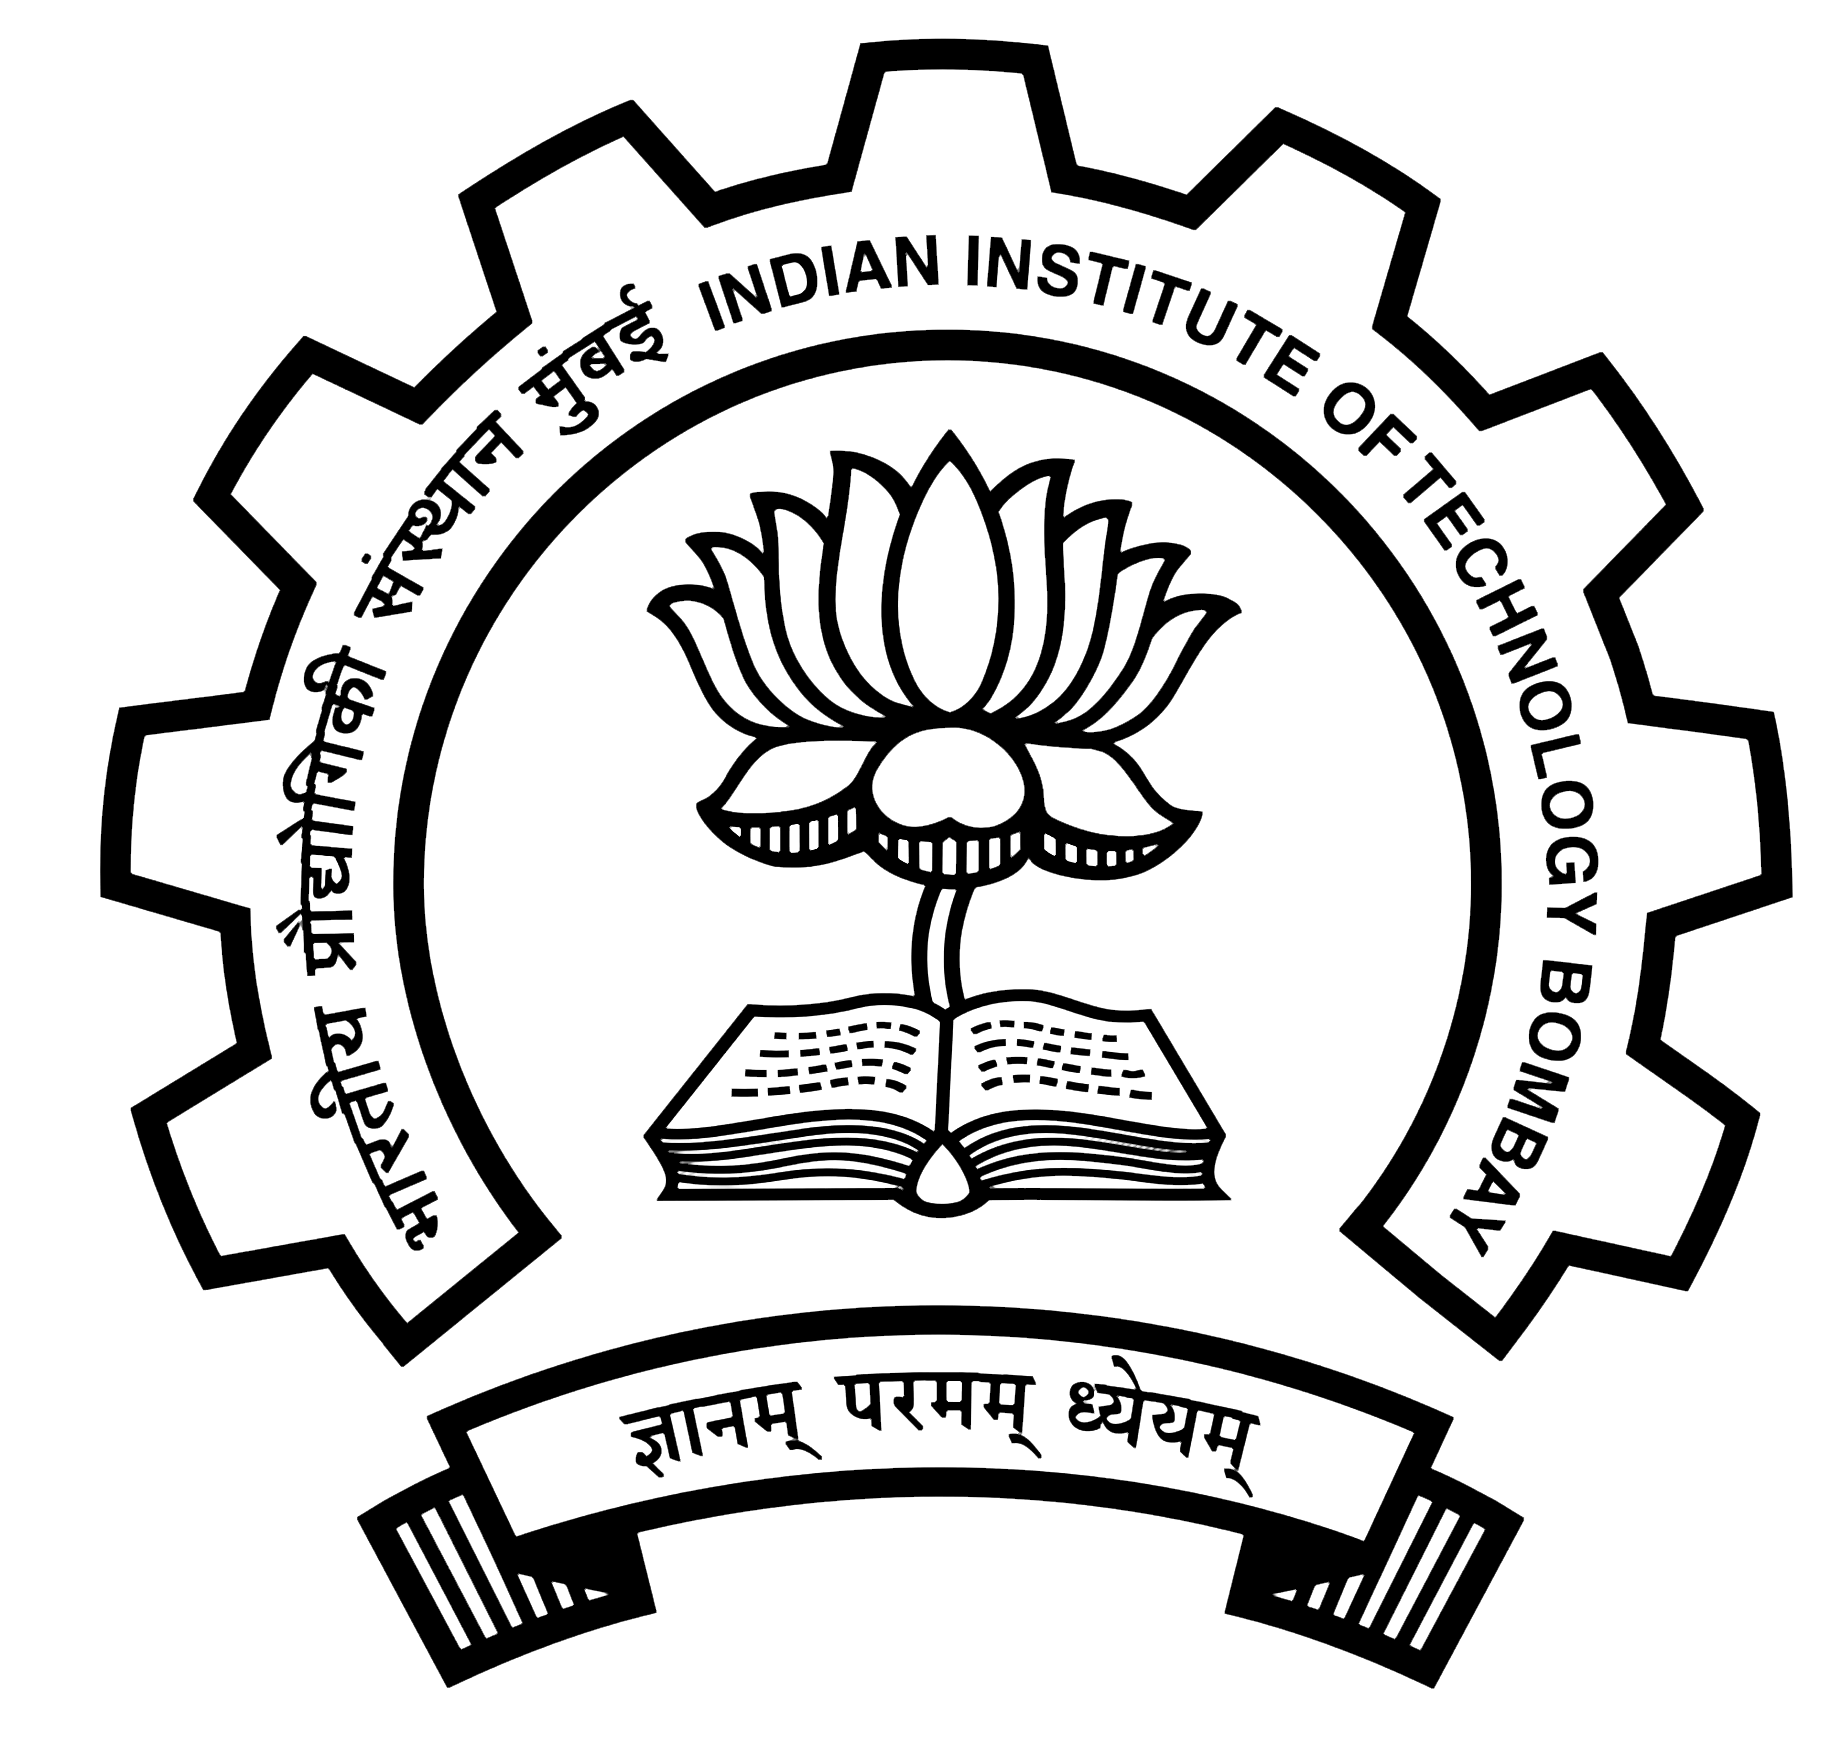
\includegraphics[width=50mm]{logo_iitb}
  \centering
  \end{figure}
  \vfill
  \large
  
Department of Civil Engineering\\
Indian Institute of Technology Bombay\\
June, 2020
\end{center}
\vfill % Fill the rest of the page with whitespace
\end{titlepage}


\pagenumbering{roman}

% \clearpage
% \thispagestyle{empty}
% \phantom{a}
% \vfill
% \begin{center}{\large \textit{This page has been intentionally left blank}}\end{center}
% \vfill

\newpage
\chapter*{Abstract}
The economy is moving towards automation. Roads are an essential factor in growth, development, and providing services. Though documented extensively in papers, the detection of small roads in mid-resolution satellites is still a problem. The work here sheds light on combining the low-level computer vision problem of super-resolution with the high-level computer vision problem of road-detection. We investigate the behavior when we first enhancing the image resolution before directly apply road-detection. We try to identify the small roads from a mid-resolution satellite image, which are otherwise skipped by the model prediction by combining the two different levels of computer vision problems.

The model uses Convolutional Neural Networks supported by ResNet architecture. It also uses encoder-decoder and dilated convolutions to segment the image to identify roads and take the spatial context into account. The method described here allows us to improve the capability of any model to now detect finer roads.


% \clearpage
% \thispagestyle{empty}
% \phantom{a}
% \vfill
% \begin{center}{\large \textit{This page has been intentionally left blank}}\end{center}
% \vfill

% \begin{center}
{\LARGE \textbf{ Declaration}}
\end{center}
I hereby declare that the matter contained in this report titled  \textbf{``Low Temperature Atomic Layer Deposition of {SiO2}"} is an authentic record of research work carried out by me at the \textbf{Devices and Interfaces Lab, Department of Energy Science and Engineering, Indian Institute of Technology Bombay, Mumbai} under the supervision of \textbf{ Prof. Shaibal K. Sarkar}, as part of the \textbf{M. Sc. - Ph. D. Dual Degree Programme} from \textbf{June 2019} to \textbf{November 2019}.\bigskip\\
I declare that this written submission represents my ideas in my own words and where others' ideas or words have been included, I have adequately cited and referenced the original sources. I declare that I have properly and accurately acknowledged all sources used in the production of this report. I also declare that I have adhered to all principles of academic honesty and integrity and have not misrepresented or fabricated or falsified any idea/data/fact/source in my submission. I understand that any violation of the above will be a cause for disciplinary action by the Institute and can also evoke penal action from the sources which have thus not been properly cited or from whom proper permission has not been taken when needed. Any oversight due to error of judgement is regretted.
\vspace{3 cm}

\begin{tabular}{p{80mm}  p{80mm}}
     Date: 20$^{\rm th}$ November 2019 &\makecell[r]{Aditya Chalishazar\\ Place: Mumbai} 
\end{tabular}


% \clearpage
% \thispagestyle{empty}
% \phantom{a}
% \vfill
% \begin{center}{\large \textit{This page has been intentionally left blank}}\end{center}
% \vfill

% \begin{center}
{\LARGE \textbf{ Certificate}}
\end{center}
This is to certify that the matter contained in this report titled \textbf{``Low Temperature Atomic Layer Deposition of {SiO2}"}  is the result of the work performed by \textbf{ Mr. Aditya Chalishazar} at the \textbf{Devices and Interfaces Laboratory, Department of Energy Science and Engineering, Indian Institute of Technology Bombay, Mumbai} under my supervision, as part of the \textbf{M. Sc. - Ph. D. Dual Degree Programme} from \textbf{June 2019} to \textbf{November 2019}.
\vspace{3 cm}

\begin{tabular}{p{80mm}  p{80mm}}
     Date: 20$^{\rm th}$ November 2019 &\makecell[r]{Prof. Shaibal K. Sarkar\\ Place: Mumbai} 
\end{tabular}


% \clearpage
% \thispagestyle{empty}
% \phantom{a}
% \vfill
% \begin{center}{\large \textit{This page has been intentionally left blank}}\end{center}
% \vfill
% \begin{center}
    \textbf{\LARGE Acknowledgement}
\end{center}
\noindent
The success of any endeavour is the contributions of several individuals.\smallskip\\

\noindent
I would like to express my sincere gratitude to my supervisor Prof. Shaibal K. Sarkar, for the opportunity to work under his guidance and his invaluable comments and suggestions regarding my work.\smallskip\\

\noindent
I owe a deep sense of gratitude to Mr. Bireswar Mandol for his continuous support in guiding my work and explaining the nuances of research work.\smallskip\\

\noindent
I extend my sincere thanks to Prof. Rangan Banerjee, the Head, Department of Energy Science and Engineering for this opportunity to be part of the M. Sc. - Ph. D. programme.\smallskip\\

\noindent
I extend my gratitude to Prof. Pratibha Sharma, Faculty Advisor for her support and suggestions.\smallskip\\

\noindent
I extend my gratitude to all other members of the laboratory: Dr. Chetan Singh, Dr. Neha Mahuli, Dr.~Anand Selvin S., Dr. Arpan Dhara, Dr. Ansuman Halder, Dr. Dayanand Sutar, Dr. Arpita Sarkar, Ms. Roja Singh, Ms. Vidya Raj, Ms. Sudeshna Ghosh, Mr. Alok Tiwari, Mr. Gaurav Bansode, Mr. Vikas Munya, Ms. Raj Rani, Ms. Shreya Sharma, Ms. Nisha Sarda, Mr. Arya Vikram for their guidance and support.\smallskip\\

\noindent
I am also grateful for the help and support of Ms. Prerna Goradia and Ms. Geetika Bajaj for their help in sample characterisation.\smallskip\\  

\noindent
I am extremely grateful for the continuous encouragement and support of my family, teachers and my friends.\smallskip\\

\noindent
I am grateful for the abundant blessings of the Almighty in every endeavor I have undertaken.

\newpage
\tableofcontents

\newpage
\listoffigures
\addcontentsline{toc}{chapter}{\numberline{}List of Figures}

\newpage
\listoftables
\addcontentsline{toc}{chapter}{\numberline{}List of Tables}

% \includepdf[pages={10}, pagecommand={}]{external.pdf}
\newpage
\addcontentsline{toc}{chapter}{\numberline{}Nomenclature}
\chapter*{Nomenclature}\label{chap:nomenclature}

\section*{Data related}
\textbf{OSM}:  Open Street Map \\
\textbf{RGB}:  Red, Green, Blue \\
\textbf{HR}:   High Resolution \\

\section*{Machine Learning related}
\textbf{AI}:   Artificial Intelligence \\
\textbf{ML}:   Machine Learning \\
\textbf{PSNR}: Peak Signal to Noise Ratio \\
\textbf{BP}:   Back Propagation \\
\textbf{SVM}:  Support Vector Machine \\
\textbf{ReLU}: Rectified Linear Unit \\
\textbf{ANN}:  Artificial Neural Network \\
\textbf{CNN}:  Convolutional Neural Network \\
\textbf{DCNN}: Deep Convolutional Neural Network \\
\textbf{SR}:   Super Resolution \\
\textbf{EDSR}: Enhanced Deep Super Resolution \\
\textbf{VDSR}: Very Deep Super Resolution \\
\textbf{FCN}:  Fully Connected Network \\

\section*{Hardware related}
\textbf{RAM}:  Random Access Memory \\
\textbf{MSI}:  Multispectral Instrument \\
\textbf{MB~/~GB}:   MegaByte~/~GigaByte \\
\textbf{GPS}:  Global Positing Systems \\ 
\textbf{GPU}:  Graphics Processing Unit \\
\textbf{TPU}:  Tensor Processing Unit \\


\pagenumbering{arabic}

%%%%%%%%%%%%%%%%%%%%%%%%%%%%%%%%%%%%%%%%%%%%%%%%%%%%%%%%%%%%%%%%%%%%%%%%%%%%%%%%%%%%%%%%%%%%
%%%%%%%%%%%%%%%%%%%%%%%%%%%%%%%%%%%%%%%%%%%%%%%%%%%%%%%%%%%%%%%%%%%%%%%%%%%%%%%%%%%%%%%%%%%%
%%%%% Text body starts here!
\newpage
\mainmatter
\chapter{Introduction}\label{chapt:intro}

Monitoring roads is an essential element in urban planning. Almost every city is developed around centers with adequate transportation facilities. They provide infrastructural support to both the agricultural and industrial sectors of every country. Given its uses in disaster management, transportation of facilities, social interaction, it is historically proven that everything can efficiently work out if we have a proper mapped site. Mapping the roads, thus, is of utmost importance.

Historically, roads were mapped manually using approximate measures, mostly for short distances, and to help religious pilgrims navigate. With the development of automobiles, maps soon became more extensive and kept in the form of books~\cite{firstMapBooks}. These were handwritten until digital maps could be produced. With the help of GPS navigation, maps started becoming digital and electronic versions were kept. These electronic versions had many advantages over their paper counterparts. Papers would quite easily be torn or lost, and this was now no longer a bugging issue. They could be replicated easily by printers or transferring files to other supported devices.

However, most of the roads in the early days were mapped using manual techniques. Taking GPS enabled devices to mark roads is both inefficient and costly. Also, some roads are inaccessible due to various factors. To combat the individual mapping of roads, Some open crowdsourcing platforms like OpenStreetMap help people continue researching by using their data. This successfully reduced the redundant work, but there is no way to check if the data is correct. Almost always, human errors reduce the quality of data. Millions of kilometers of roads are still left to be digitalized to be used for any activity~\cite{MapsDoneOSM}. Even if we complete mapping of the remaining roads, It still does not guarantee us the latest report as previous road data might have changed.

The computer is one piece of technology which makes our work a lot simpler. With the advent of techniques such as Machine Learning, identifying patterns to solve certain kinds of Problems has become a lot easier. The work here is an attempt to use image segmentation based on computer vision techniques to detect roads in satellite images. This will help in reducing the manual workforce to a large extent. While many road detection papers are available, these papers mostly focus on identifying roads while the camera is on the road. While this has it's own uses in navigation, but using these techniques for surveying is not feasible as one will have to drive all the way, resulting in highly inefficient surveying. Some papers have tried to overcome this problem by high-resolution satellite images, but high-resolution images are quite expensive and have to be bought commercially. Another widespread problem these satellites face is radiometric distortion. Roads of asphalt, sometimes turn from dark grey into bright white due to some reflection affecting satellite sensors. This is seen clearly is Figure~\ref{fig:sat_img_radiometric_distortion}~\cite{GF2-imageCaseStudy}.

\begin{figure}[h!]
  \centering
  \begin{subfigure}{0.48\textwidth}
    \includegraphics[width=\textwidth]{sat_img_GF2_radiometric_distortion}
    \caption{}
  \end{subfigure}~
  \begin{subfigure}{0.48\textwidth}
    \includegraphics[width=\textwidth]{sat_img_zoomed_GF2_radiometric_distrotion}
    \caption{}
  \end{subfigure}
  \caption[Optical distortion clearly visible on roads]{Optical distortion clearly visible on roads. (a) Radiometric distortion in image from GF2 satellite (b)~Zoomed image of (a). Taken from~\cite{GF2-imageCaseStudy}.}
  \label{fig:sat_img_radiometric_distortion}
\end{figure}

Road detection using satellite data is already tough due to the many discontinuities arising given large tree canopies or due to being overshadowed by buildings. Road detection using a mid-resolution satellite is tougher, given the resolution is usually around 1~m-10~m. A typical two-lane road has a width of around 7~m, and this width in the best case is just depicted by just 7 pixels, leave out the worst case where a pixel hardly shows a road. The work here is an effort to use the valuable image segmentation techniques into the area of remote sensing to detect roads in mid-resolution satellite images.
\chapter{Problem definition and background}\label{chapt:problem}
Road digitalization is an expensive operation. Research is being done to identify roads automatically using Artificial Intelligence~(AI) with the different types of images. High-resolution satellite images are expensive to get, and covering an entire state or country is a nightmare. On the other hand, mid-resolution satellite images can be obtained for free, but the identification of roads on mid-resolution~(>~5~m) satellite data is difficult and often has low accuracy. This work tries to detect the smaller roads~(with 1 or 2 lanes), which are often missed.

We will be using RGB images from satellite Sentinel-2A. \Cref{tab:sentinel-resolution} lists the detailed parameters of the satellite. Band 2 (Blue), 3 (Green), and 4 (Red) are stacked together to get a 3-channel RGB image. As seen in the specifications, the spacial resolution of the final image is 10~m. The task is to increase the accuracy of the existing road-detection algorithm.

\begin{table}[h!]
  \centering
  \begin{tabular}{ |c|c|c| }
    \hline
    Spatial resolution~(m) & Band number & Central wavelength~(nm) \\
    \hline
    10&2&492.4 \\
    10&3&559.8 \\
    10&4&664.6 \\
    10&8&832.8 \\
    20&5&704.1 \\
    20&6&740.5 \\
    20&7&782.8 \\
    20&8a&864.7 \\
    20&11&1613.7 \\
    20&12&2202.4 \\
    60&1&442.7 \\
    60&9&945.1 \\
    60&10&1373.5 \\
    \hline
  \end{tabular}
  \caption[Wavelengths and bandwidths of the three spatial resolutions of the MSI instruments]{Wavelengths and bandwidths of the three spatial resolutions of the MSI instruments~\cite{sentinelSpecifications}}
  \label{tab:sentinel-resolution}
\end{table}

By combining the three bands from the raw satellite image, the resulting image size is of the order of 400~MB for one mid-sized city. At first, this may not seem significant in comparison with some of the media files. Yet, handling files of this size in DCNN is a severe issue. Processing large files might be possible for massive supercomputers; however a general workstation has Random Access Memory~(RAM) anywhere from 128 to 256~GBs of RAM, while personal computers range from 8~GB to 32~GBs of RAM. Thus, this image must be divided into several parts so that our algorithms work on a readily available device.

Our input image does not have a sufficiently high resolution to identify small roads. To deal with this problem of pixelization, we will be using two types of models. This setup is shown in \cref{fig:model_complete_without_labels}. Unless specifically mentioned, a model means a combined setup using super-resolution and road-detection models. Data from the input layer goes to the super-resolution model, which is consequently passed to the road-detection model. The final output consists of the predicted road network in the image.

\begin{figure}[h!]
  \centering
  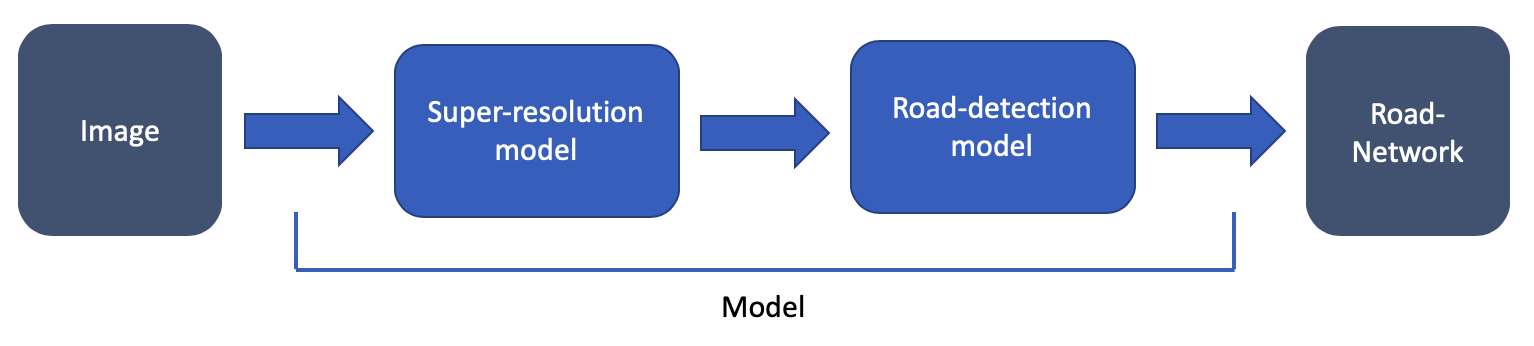
\includegraphics[width=\textwidth]{model_complete_without_labels}
  \caption{Complete setup: Combination of super-resolution and road-detection models.}
  \label{fig:model_complete_without_labels}
\end{figure}

\chapter{Previous work}\label{chapt:previous}
\textit{The idea of using satellite data has been researched within many communities. Several automated and semi-automated ways are proposed to tackle the problem of detecting roads. These ways are quite different due to the different strategies and algorithms used by them. The different strategies come into the picture to tackle the various challenged like noisy data, occlusions, distortion and complex backgrounds which appears in images.}

\section{Road detection}
The journey to digitally identify the roads started with the topic of reducing cost and increasing productivity. One of the first road detection algorithms were static methods and focused on the color and geometry of roads. These methods were quite unreliable, mainly because of the discontinuities arising due to the similar color range of roads and shadows~\cite{Detecting_interections_using_color,Detecting_roads_using_color}. Another disadvantage was the need for high-resolution images (ca 0.2~m~-~0.5~m), which is hard to get. The idea was then improvised to include texture cues for road detection~\cite{using_texture_for_road_detection,baumgartner1999automatic}. The accuracy was indeed better, but the need for a very high-resolution image remained a problem. With the machine learning techniques, the pixel-level classification started to give improved performance~\cite{road_detection_using_neural_nets_SVM,road_detection_using_env_learning,road_detection_using_SVM_online_learning}.

The Support Vector Machine~(SVM) methods have a good generalization ability and thus are widely used in object detection from a given image. They are, at most times, more accurate and give consistent robust results than other classification techniques such as K-nearest neighbor. Nevertheless, the estimation of kernel functions and the choice of the dimensional space and training samples led to the SVM classifier~\cite{YagerSowmya2003,melgani2004classification}. This was done using edge-based features such as gradient, intensity, edge length, and classified objects in a high-resolution image. SVM approaches are well suited for multispectral data, where we have an adequate number of vectors to classify objects~\cite{Simler2011}.

In 2003, Tu-Ko presented a robust approach, in which a back-propagation~(BP) neural network was trained with the spectral and edge information to find the road centerline. Although errors prop in, the model was still useful as a whole. Disadvantages of BP neural network include slow convergence speed, the need for an extensive training data set, inability to find global minima, and over-fitting risks. Since then, many types of neural networks like fuzzy neural networks~\cite{mokhtarzade2008automatic} and Convolutional Neural Networks~(CNN) have been used to capture the spacial contexts of road networks, giving much better accuracies on fewer resources.

With the developments of Graphics Processing Units~(GPUs) and Tensor Processing Units~(TPUs) and the progress of ResNet architectures, even Deep Convolutional Neural Networks~(DCNN) have been researched and changed the way road extraction works. The recent developments with encoder-decoders, dilations, and fuzzy logic have inspired state-of-the-art algorithms like UNet, SegNet, LinkNet, and its further improvements like D-LinkNet and AD-LinkNet~(\cref{fig:compare_road}). Moreover, competitions pitch in the researchers by providing them with a precise dataset and motivating them to thrive and excel in the world race.

\begin{figure}[h!]
  \centering
  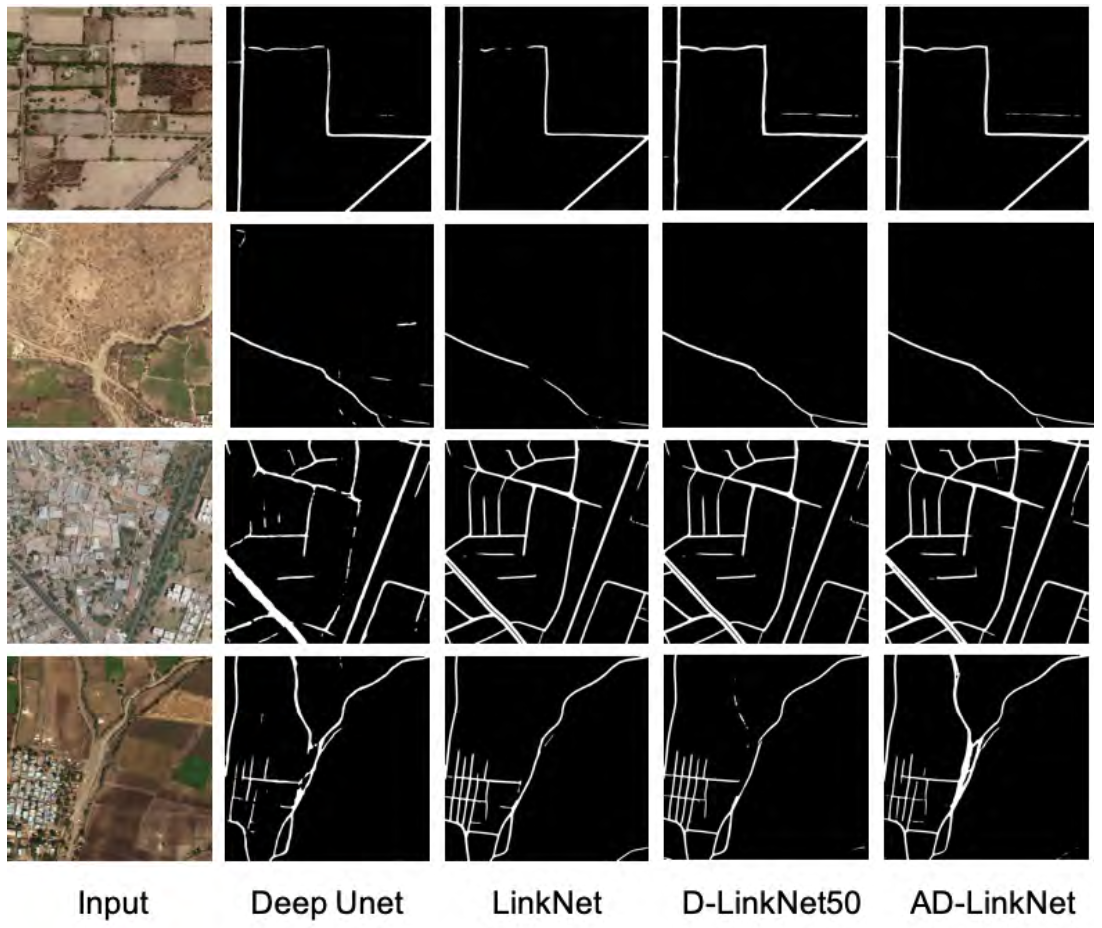
\includegraphics[width=\textwidth]{compare_road}
  \caption[Comparison of different road-detection models]{Comparison of different road-detection models. Adapted from~\cite{AD-LinkNet}}
  \label{fig:compare_road}
\end{figure}


\section{Super Resolution~(SR)}
Many models have proposed methods to obtain a super-resolution image from the given image. Most of the techniques use bicubic upsampling of the image as an input to the proposed neural network model. However, this was inefficient as a significant part of memory is required for performing bicubic upsampling. The authors of~\cite{EDSR} additionally questioned the architectural optimality used in the existing networks. Though neural networks provide significantly improved performance in terms of peak signal-to-noise ratio (PSNR) in the SR problem, it is also proven to be quite sensitive to minor architectural changes. The outputs differ in performance with different training techniques. The authors further proposed an enhanced deep super-resolution network (EDSR) with performance exceeding the past state-of-the-art super-resolution models. This was achieved by carefully designing model architecture using sophisticated optimization methods in training the neural networks.

Secondly, the authors noticed that most existing models treat the super-resolution of different scale factors as an independent problem. There is no consideration of learning the mutual relationship between different scales. With efforts such as the development of Very Deep Super Resolution~(VSDR), this relationship is proved to be feasible and much more accurate than the single-scale models, though at the cost of heavier computation time and memory utilization. Further work was restricted by a lack of ability to use very deep neural networks.

With the break-through changes brought by concepts of skip-connects and residual blocks, neural networks were shown to be trained with 100+ layers. SRNet solved incorporated the ResNet architecture and solved the problem of high memory utilization. Because ResNet architecture was proposed to solve higher-level computer vision problems such as image classification and detection, its use directly for a low-level problem like computer vision can be optimized.

EDSR proposes using a modified type of residual block to remove the unnecessary elements and optimize the model's performance. Secondly, a new architecture is used with fewer parameters but showing comparable performance. \Cref{fig:compare_SR} shows a comparison between different SR algorithms.

\begin{figure}[h!]
  \centering
  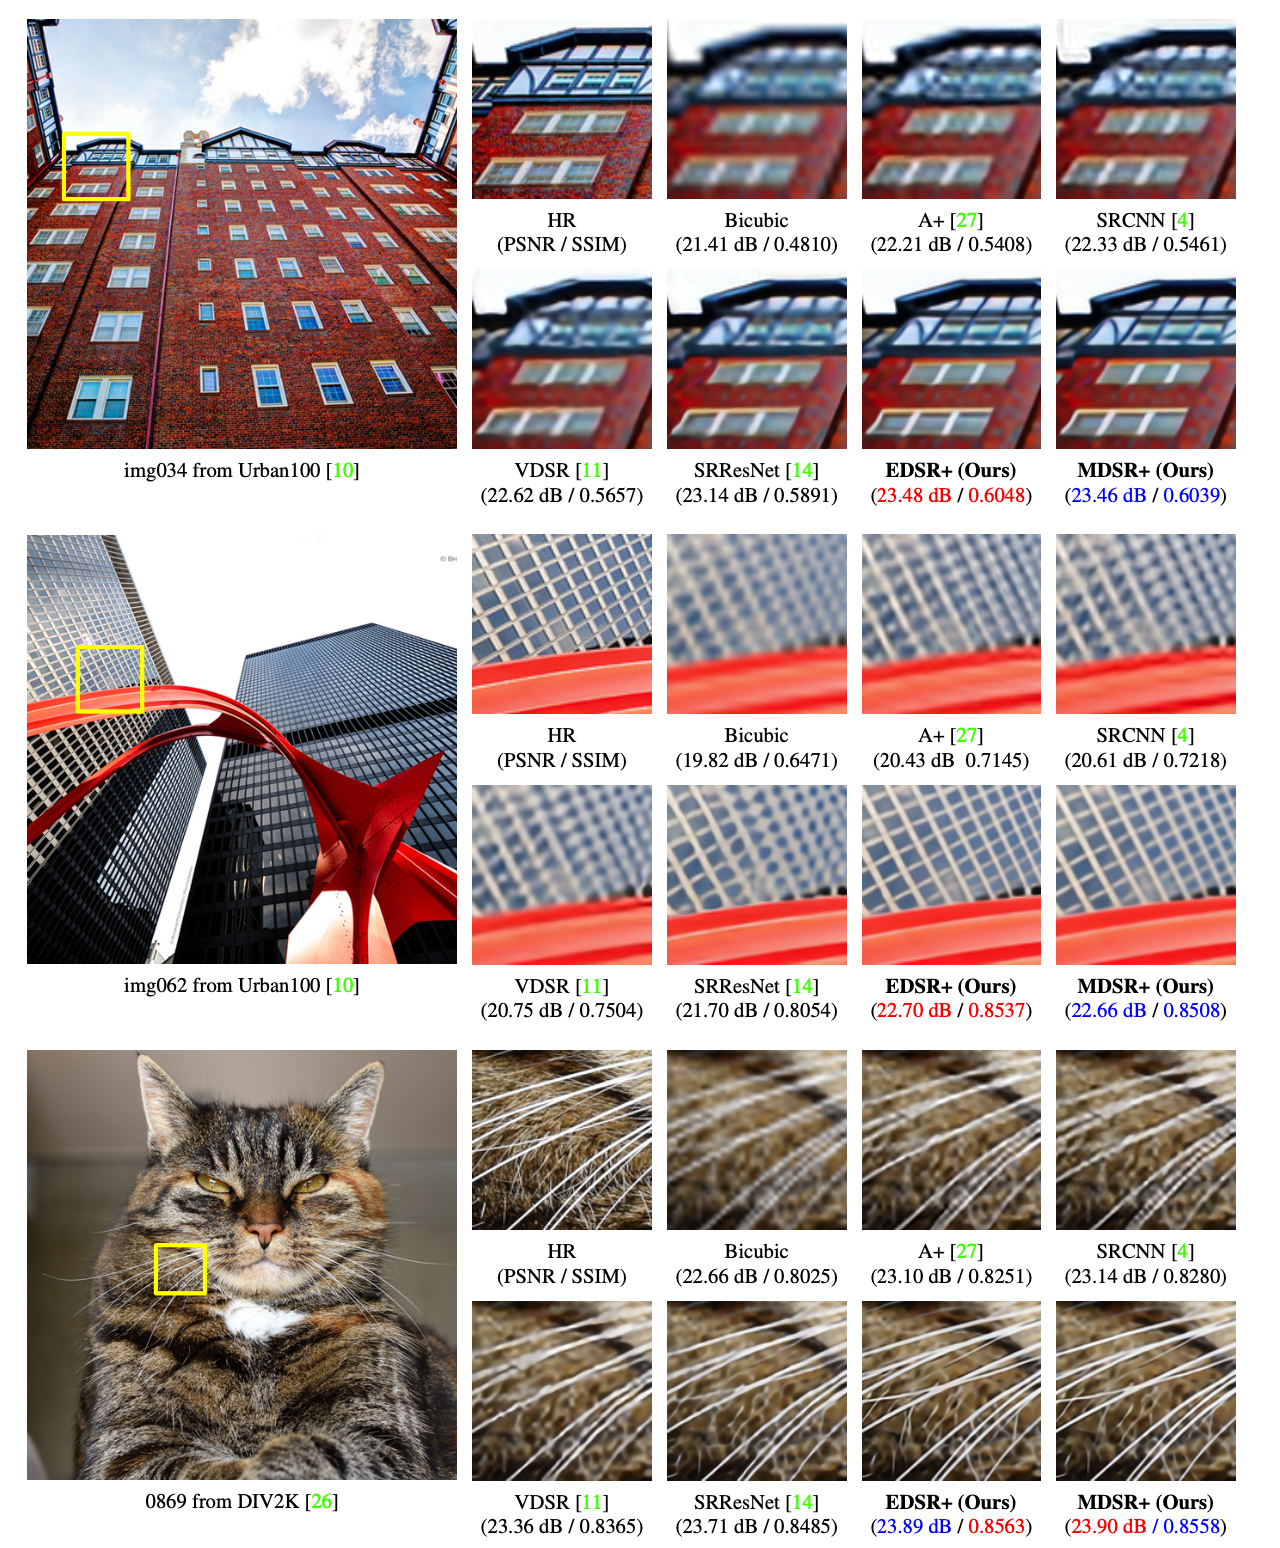
\includegraphics[width=\textwidth]{compare_SR}
  \caption[Comparison of different super-resolution models]{Comparison of different super-resolution models. HR is raw high resolution image taken. Adapted from~\cite{EDSR}}
  \label{fig:compare_SR}
\end{figure}

\chapter{Literature review}\label{chapt:lit}
\section{Convolutional Neural Networks(CNN)}
[\textit{A CNN is a type of Artificial neural network(ANN) where convolutional blocks are used instead of basic 1-D multilayer perceptrons}]

For understanding CNN, we need to see what an artificial neural network(ANN) is. ANN is a system of interconnected neurons used to model complex functions for classification and regression. Any model is made up of at least three layers: An input layer, one or more hidden layers, and an output layer. The most basic ANN model consists of multilayer perceptrons. \ref{subsection:types_of_layers} shows different types of layers that can be used for a convolutional neural network. Several nonlinear activation functions such as rectified linear unit (ReLU)or sigmoid, or even custom functions can be applied at any point on the layers to produce activation maps. These activation maps finally help us in classification or segmentation.

\subsection{Types of layers}
\label{subsection:types_of_layers}
The general structure of any convolutional neural network can be categorized as follows:
\begin{enumerate}[(a)]
    \item \textbf{Input layer}:
        The input layer is the input of any neural network. The input of computer vision problems is usually an image that is basically a matrix of numbers stacked multiple times(channels). An RGB image has 3 channels[Figure~\ref{fig:RGB_image}].
        \begin{figure}[h!]
            \centering
            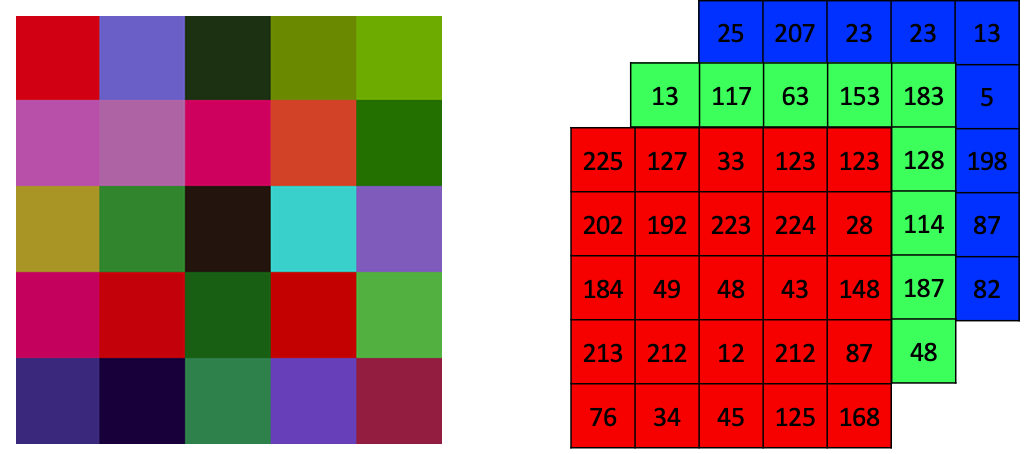
\includegraphics[width=0.8\textwidth]{rgb_image_as_array}
            \caption[RGB image shown as matrix]{RGB image shown as matrix. Resolution of this image is $5\times5$.}
            \label{fig:RGB_image}
        \end{figure}
        
    \item \textbf{Convolution layer}:
        As the name suggests, this is the most important layer of convolutional neural networks. A convolutional layer contains a set of filters(or kernel or node) whose parameters need to be learned. The height and width of the filter are predefined when defining the layer and are smaller than those of the input volume. For most images, the dimension of the filter is taken $3\times3$ or $5\times5$, but if the given image is large, filters up to size $11\times11$ can also be used. One catch is: a filter is not two dimensional. It takes in the dimension of the input it is provided with.

        Applying a filter to an image means taking the inner product of the image and the filter within the overlapping area, which keeps on moving. Suppose the dimension of an image is $W\times W$ and dimension of the filter is $k\times k$, the dimension of the output image will be $(W-k+1)\times (W-k+1)$. Once a filter has been applied, it passes through an activation function, and the resulting image is called the output of that filter.
    
        The formula for convolutional neural network is: \begin{equation} a_{i,j} = f(\Sigma_{m=0}^2\Sigma_{n=0}^2 W_{m,n}X_{m+i,n+j}) \end{equation} where $\text{X}_{i, j}$ represents the pixel value of line $i$ in column $j$ of the image and $W_{m, n}$ represents the weight of column $n$in row $m$. Similarly, $a_{i,j}$ represents the value of column $j$ of the $i$ row of the feature map; the activation function is represented by $f$. [Example: Figure~\ref{fig:convolution_filter_process}].
        \begin{figure}[h!]
            \begin{subfigure}[b]{0.35\textwidth}
            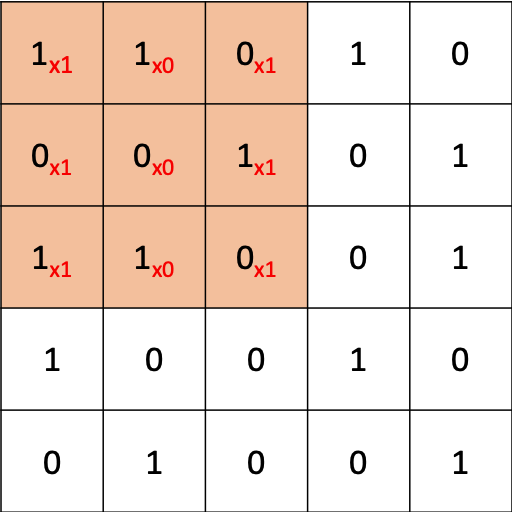
\includegraphics[width=\textwidth]{cnn_filter_input}
            \caption{}
            \end{subfigure}~
            \begin{subfigure}[b]{0.2\textwidth}
            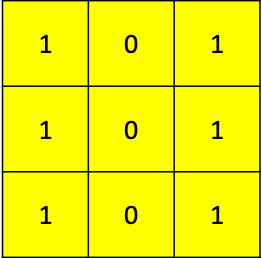
\includegraphics[width=\textwidth]{cnn_filter}
            \caption{}
            \end{subfigure}~
            \begin{subfigure}[b]{0.2\textwidth}
            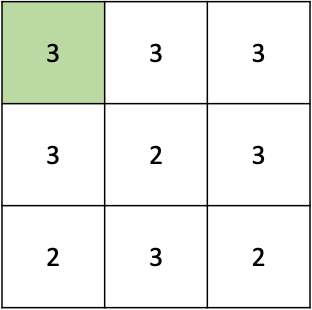
\includegraphics[width=\textwidth]{cnn_filter_convolution}
            \caption{}
            \end{subfigure}~
            \begin{subfigure}[b]{0.2\textwidth}
            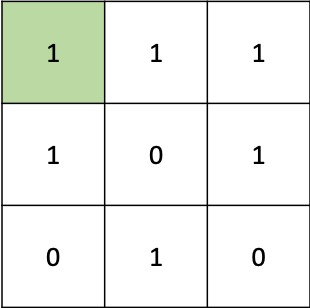
\includegraphics[width=\textwidth]{cnn_filter_output}
            \caption{}
            \end{subfigure}
            \caption[The process of convolution]{The process of convolution: (a) Input vector. (b) Filter being convoluted on (a). (c) Result of (b) convoluting over (a). (d) Final result after applying activation function $a_{i,j}>2$.}
            \label{fig:convolution_filter_process}
        \end{figure}

        Each filter in the convolution layer uses the output of the previous layer to connect and calculate. The number of filters is predefined and usually kept in powers of 2. Suppose a layer has 64 filters of dimension $3\times3$, the input image has dimensions of $1000\times1000$, the resulting output will be of dimension $998\times998\times64$. If this is passed into another layer consisting of 128 filters and the same dimension, the new output will be $996\times996\times128$.

    \item \textbf{Pooling layer}:
        The amount of data after the multilayer convolution layer is huge. To reduce the time taken for calculations, we need to reduce the size of the matrix. This means we need to reduce the number of parameters of the fully-connected layer. This is done by using a pooling layer. The pooling layer finds the eigenvalues of the image, which are then used as the basis of classification. The pooling layer also prevents data from overfitting.

        The pooled layer function similar to data resampling. The filter propagates in the same way as the filters in the convolution layer. The difference between the two is that instead of taking the inner product with the filter, we take the maximum or average value of the window. The most used pooling methods are max pooling, mean pooling, and random pooling layers. In a max-pooling layer, the maximum value of a pre-specified window replaces the given dataset. If the dataset is replaced by averaging the contents in the window, it is called an average pooling layer. A number is selected randomly according to the probability matrix in random pooling.

    \item \textbf{Fully connected layer}:
        Unlike the filters in the convolution layer where only some pixels are taken into account, each fully connected layer uses the previous layer's global information. This means each node’s calculation is connected with the weights of all nodes in the previous layer. This is the reason this layer is usually used at the end of the model. 

        Because it takes in the global context, this means the complete information received from convolution and pooling operations is taken into consideration for output from this layer. Given the outputs, an activation function is applied for classification purposes.
\end{enumerate}

% TODO: There are some special types of convolutional layers which perform specific tasks:
\subsection{Dilated convolution}
[\textit{Convolution with dilated filter; Also called atrous convolution}]

    Dilated convolutional layers are used in image segmentation, where its class labels each pixel. As the name suggests, Dilated convolution is basically dilating the filter before doing the usual convolution. Dilating the filter means expanding, taking in distant elements instead of the adjacent elements in the input matrix to calculate weights. These filters are also called upsampled filters. The empty positions in between are filled with zeros, thus making this kind of sparse matrix. The distance in a Dilated convolution filter is determined by the dilation coefficient D(Also called dilation rate). If the dilation rate is 1, it means it is the standard convolutional kernel. If the dilation rate is 2, then there is a skip of one pixel per input. In general, if there is a dilation rate of n, skip of n-1 pixels per input.
    
    Figure~\ref{fig:dilated_layer} shows how the kernel elements are matched to input elements in a D-dilated 3x3 convolution. Also notice how the dilated convolution layer has increased the spatial context(a.k.a feature maps or receptive field or the field of view) without decreasing the resolution of output.
    \begin{figure}[h!]
        \centering
        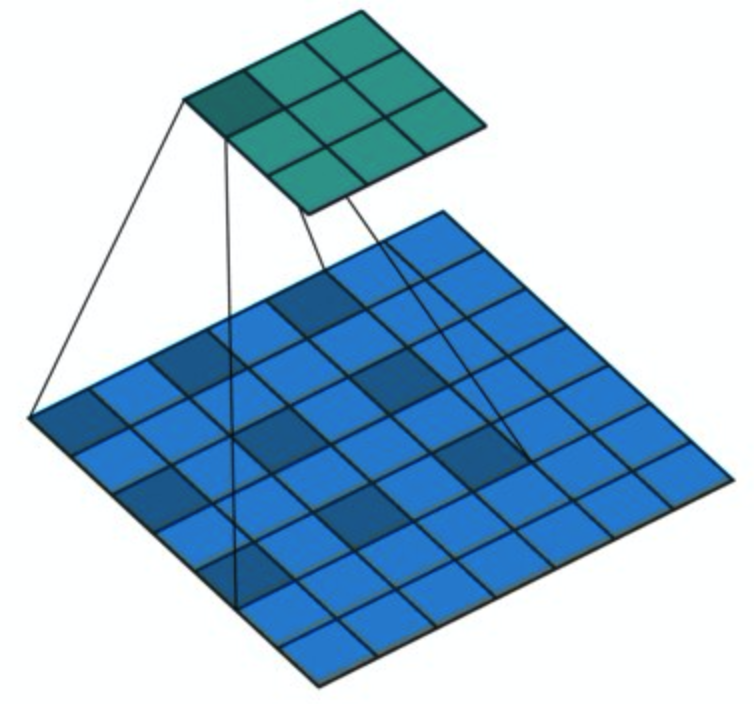
\includegraphics[width=0.5\textwidth]{cnn_dilated_layer}
        \caption[Dilated convolution layer]{Notice how dilated convolution layer increases the capture of spatial context. Dilation rate is 2 in this figure.}
        \label{fig:dilated_layer}
    \end{figure}


\subsection{Strided convolution}
    In a regular convolution, we usually shift the windows by 1 pixel. However, for some large images, it is necessary to shrink feature maps to make computations feasible. In stride convolution, we change the length of stride in each step. This means we skip some input values while performing convolution operations and thus decreasing the output dimension. In general, this operation does a trad off between resource consumption and information retrieval.


\section[Residual Networks]{Residual Networks}

In a neural network, weights receive an update proportional to the gradient of current weight in each iteration. \begin{equation} ChangeInWeight_{i} \propto \frac{\partial(ErrorFunction)}{\partial(weight_{i})} \end{equation} When the gradient of the training model becomes vanishingly small, the change in weight becomes negligible, and thus model training essentially stops. This problem is called the problem of vanishing gradient.

Conventionally, as the CNNs become deeper, the problems related to vanishing gradients became severe. To solve this problem, {Kaiming He, Xiangyu Zhang, Shaoqing Ren, Jian Sun}\cite{ResNet} developed the concept of residual networks(Also called ResNet or skip connections). Residual neural networks tackle vanishing gradients by skipping connections or making shortcuts to jump over some layers (Figure~\ref{fig:residual_network}). Typical ResNet models are implemented with double- or triple- layer skips that contain nonlinearities (ReLU) and batch normalization in between.

\begin{figure}[h!]
    \centering
    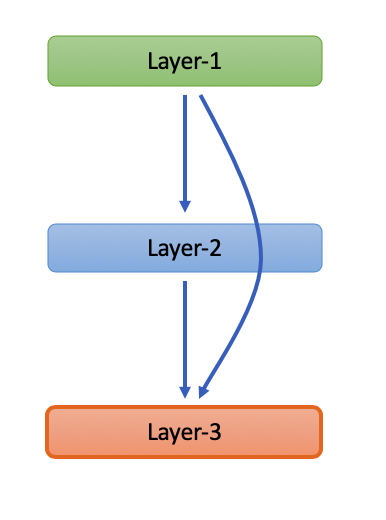
\includegraphics[width=0.2\textwidth]{lit_resnet}
    \caption[A residual network]{Canonical form of a residual neural network. Layer-2 is skipped over activation from Layer-1.}
    \label{fig:residual_network}
\end{figure}

While training, an additional matrix can be used to train the skip connections as well. These are usually identity matrices and not so hard on memory; hence they can be used to quickly train much deeper networks than what was achieved with the conventional neural networks. ResNet also increases performance while training the model. This is due to the face that some layers are essentially skipped, and the gradients that were earlier vanishing now converge faster.

Many improvements to the original ResNet architecture have been made since its inception. Pre-trained models like ResNet (34, 50, 101) are already available in popular libraries like Tensorflow and PyTorch. ResNet is considered one of the most significant innovations in the area of neural networks

\section{Encoder-Decoder}
The encoder-decoder architecture is the standard neural machine translation method that rivals and, in some cases, outperforms classical statistical machine translation methods.

Though this architecture is very new, having only been pioneered in 2014. The Encoder-Decoder architecture has become a modern approach for sequence-to-sequence (seq2seq) predictions. Road detection needs a sequence-to-sequence learning framework to keep track of spatial characteristics. It has three components: an encoder network, a decoder network, and an intermediate network.

The encoders are trained with the decoders. There are no labels (hence unsupervised). The loss function is based on computing the delta between the actual and reconstructed input. The optimizer will try to train both encoder and decoder in such a way that the features that matter the most should have lower reconstruction loss. This also means that, given an encoded sequence, we do not try to reconstruct the actual input, but rather try to map inputs to specific outputs. For example, given a map, it maps roads to true and assigns everything else to false. This is how a Lossy compression algorithm helps us in the segmentation of an image.

% \section{Super Resolution}


% \section{Road Detection}
% It can be both binary and fuzzy

% \section{Training process of convolutional neural network}

% In this paper, the road extraction of remote sensing image is studied. Firstly, the convolutional neural network is used to classify the high-resolution remote sensing image, distinguish the road from the non-road, and extract the road information initially. Secondly, the convolutional neural network is optimized and improved from the training algorithm. In this section, the training process of convolutional neural network is improved to realize road classification in remote sensing images.

% Gradient descent algorithm is simple, easy to converge, but easy to fall into the local optimal solution, and the gradient descent near the saddle point is slow, affecting the training of network model. The saddle point can be avoided in the training process of Newton algorithm, but the method needs to compute Heisen matrix to ensure its non-negative positive definite and a large amount of storage space and to ensure the existence of second-order derivatives of the objective function; otherwise, it is difficult to ensure the convergence of the algorithm [26,27,28]. In order to avoid the difficulties caused by the direct use of the Newton algorithm, the improved BFGS quasi-Newton algorithm [29] is used to train convolutional neural networks.

% In the Newton algorithm training process, the CNN model parameters are updated to:
% 𝑊𝑖+1=𝑊𝑖−∇𝑗𝑤∇2𝑗𝑤
% (9)

% The initial quasi-Newton algorithm equation is:
% 𝐵𝑘+1𝑆𝑘=𝑦𝑘
% (10)

% where Sk = Wk + 1 − Wk, yk =  ∇ jw + 1 −  ∇ jw. In order to achieve better target optimization effect, the improved BFGS is used in this paper.
% 𝐻𝑘+1=𝐻𝑘+𝑦𝑘𝑦𝑡𝑘𝑦𝑡𝑘𝑠𝑘−𝐻𝑘𝑠𝑘𝑠𝑡𝑘𝐻𝑘𝑠𝑡𝑘𝐻𝑘𝑠𝑘
% (11)

% However, the Heisen matrix obtained by the recursion formula may be a singular matrix, and the inverse matrix calculation has a certain degree of complexity, so the recursion formula in this paper is expressed as follows:
% 𝐵−1𝑘+1=(𝐵0−𝑠𝑘𝑦𝑇𝑘𝑠𝑇𝑘𝑦𝑘)𝐵−1𝑘(𝐵0−𝑦𝑘𝑠𝑇𝑘𝑠𝑇𝑘𝑦𝑘)+𝑠𝑘𝑠𝑇𝑘𝑠𝑇𝑘𝑦𝑘
% (12)

% Based on the above theory and formula, the training process of the improved BFGS algorithm is as follows:

%     1.

%     Select iteration times epochs, epoch = 0, initialization parameter w and offset b.
%     2.

%     If epoch < epochs, iteration stops.
%     3.

%     Calculate the value of bkdk +  ∇ jw = 0 and get a new optimization direction 𝑑𝑘=−𝐵−1𝑘𝑔𝑘

%     .
%     4.

%     Search along the dk direction to satisfy wk + 1 = wk + akdk, it is the minimum point in this direction, ak > 0.
%     5.

%     Let the epoch iteration add 1 and go to (2).

\chapter{Proposed computational model}\label{chapt:model}
\textit{By combining the power of \textbf{(a)} Super-resolution: EDSR and \textbf{(b)} D-LinkNet and taking care of noise during training, we enhance the accuracy of our deep learning model.}

\section{Super-resolution: EDSR}
Our input image does not have sufficiently high resolution to identify small roads. To solve this problem, we use the concept of super-resolution. We plan to use the EDSR model~\cite{EDSR} for this project. This model is based on a modified ResNet architecture. This is because the original ResNet architecture is made taking high-level computer vision problems in mind~\cite{khan2019surveyResNet}. In simple words, ResNet architecture might not be so efficient for a model that does not deal with features but use a general pattern to upsample an image~(low-level computer vision problem). 

The model consists of a $3\times3$ convolution layer, which passes information into two modified residual blocks. The output is again sent to a $3\times3$ convolution layer. This entire block is skipped over by directly adding the input image with the block output. The resultant matrix is sent to an upsample block and a convolution layer to get the resultant.

The proposed residual block is fairly simple and is simply two convolution layers with a ReLU activation function in between them. The output is added to the input given to the block, thus taking advantage of skip-connections.

The upsample layer has a convolution and a shuffle layer in an alternating fashion. The shuffle layer is needed to ensure that the learning does not learn any features to cause bias in upsampling. The features might be color-based, edge-based, pixel-based, or some intricate learned pattern.

The model as proposed is shown in \cref{fig:model_EDSR}.

\begin{figure}[h!]
  \centering
  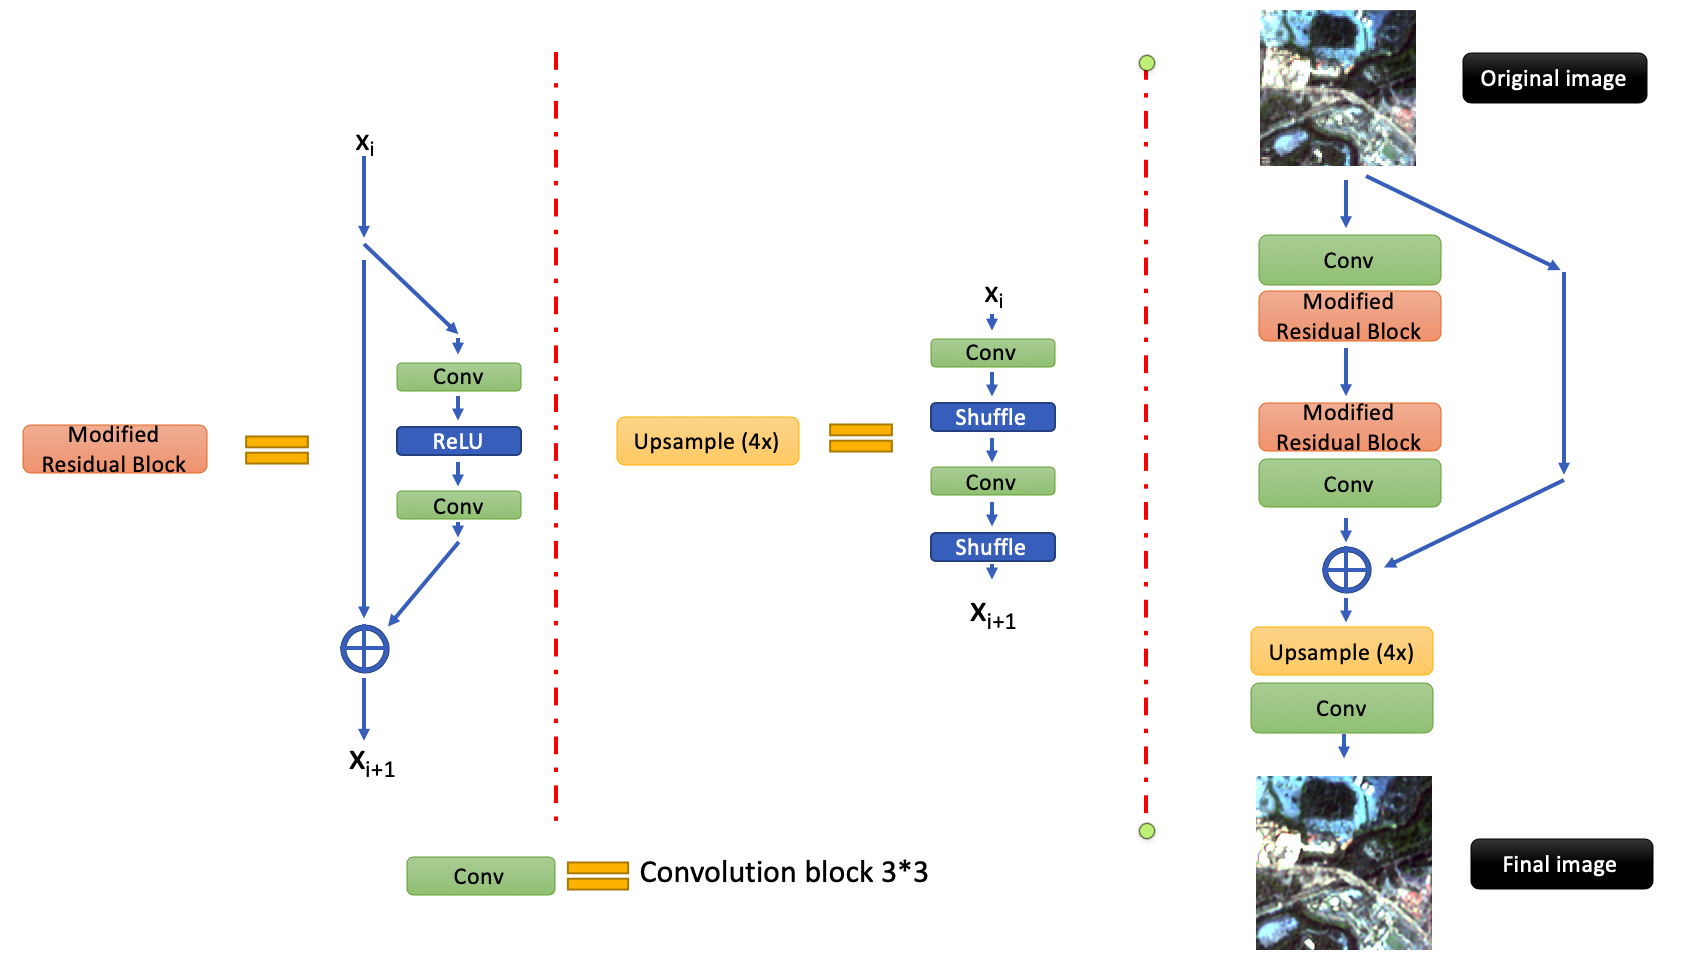
\includegraphics[width=\textwidth]{model_EDSR}
  \caption[Laying out the strucutre for EDSR]{Laying out the strucutre for EDSR~\cite{EDSR}.}
  \label{fig:model_EDSR}
\end{figure}


\section{D-LinkNet: Finding the road networks in the image}
As opposed to super-resolution, road detection is a high-level computer vision problem. It involves finding a relationship between features and taking into consideration the spatial context for road-connectivity. In D-LinkNet, the road extraction task is taken as a binary task to generate pixel-level labeling of roads while considering neighborhood pixels. Going with deep learning models, we can classify the data by learning the weights during the training phase. However, roads are connected and spatially continuous. To ensure this continuity, we use dilated layers to ensure we store data in weights. Directly using a Fully Connected Network~(FCN) is also an option, but the memory requirement for any image is huge to be executed in a practically feasible way.

\subsection{Extracting the essential features}
Considering a large image, we start with a convolution layer with a big window to say $7\times7$. To further reduce the computational load, a pooling layer is used. Now that we have some manageable representation of the image in a matrix, we start with our actual model. Road detection is a complex task and has many features to be captured. As the number of features increases, we make the CNNs deeper. We use the ResNet architecture to make sure vanishing gradients do not stop us from training a deep CNN model. I used multiple residual blocks and used a pooling layer whenever I felt the data becoming overwhelmingly large. Every time before a pooling layer, I added the output to the input to make sure the image's data is not lost.

On a trial and error basis, after some 50 convolution layers, it is seen that features are separated. To separate the features, and identify the roads, an encoder-decoder architecture is used. It accepts a single element of the input sequence, processes it, collects information from that element, and propagates it to the next step. This means that when the encoding is complete, the entire information is available in the intermediate step.

\subsection{Taking into consideration the spatial connectivity of roads}
Before decoding the output, during the intermediate step, we gather data to ensure connectivity using dilated convolution layers. Dilated convolution layers enlarge the receptive field of feature points without reducing the resolution of the image~(Refer \cref{sec:Dilated_Convolution}). Using multiple dilations convolution layer ensures we have spatial context from multiple different neighborhoods.

As we have the complete sequence available, we use the decoder to decode the sequence we had encoded. Using the encoder-decoder enables us to segment the image to make accurate predictions easily.

The model proposed is given in \cref{fig:model_D-LinkNet}.
\begin{figure}[h!]
  \centering
  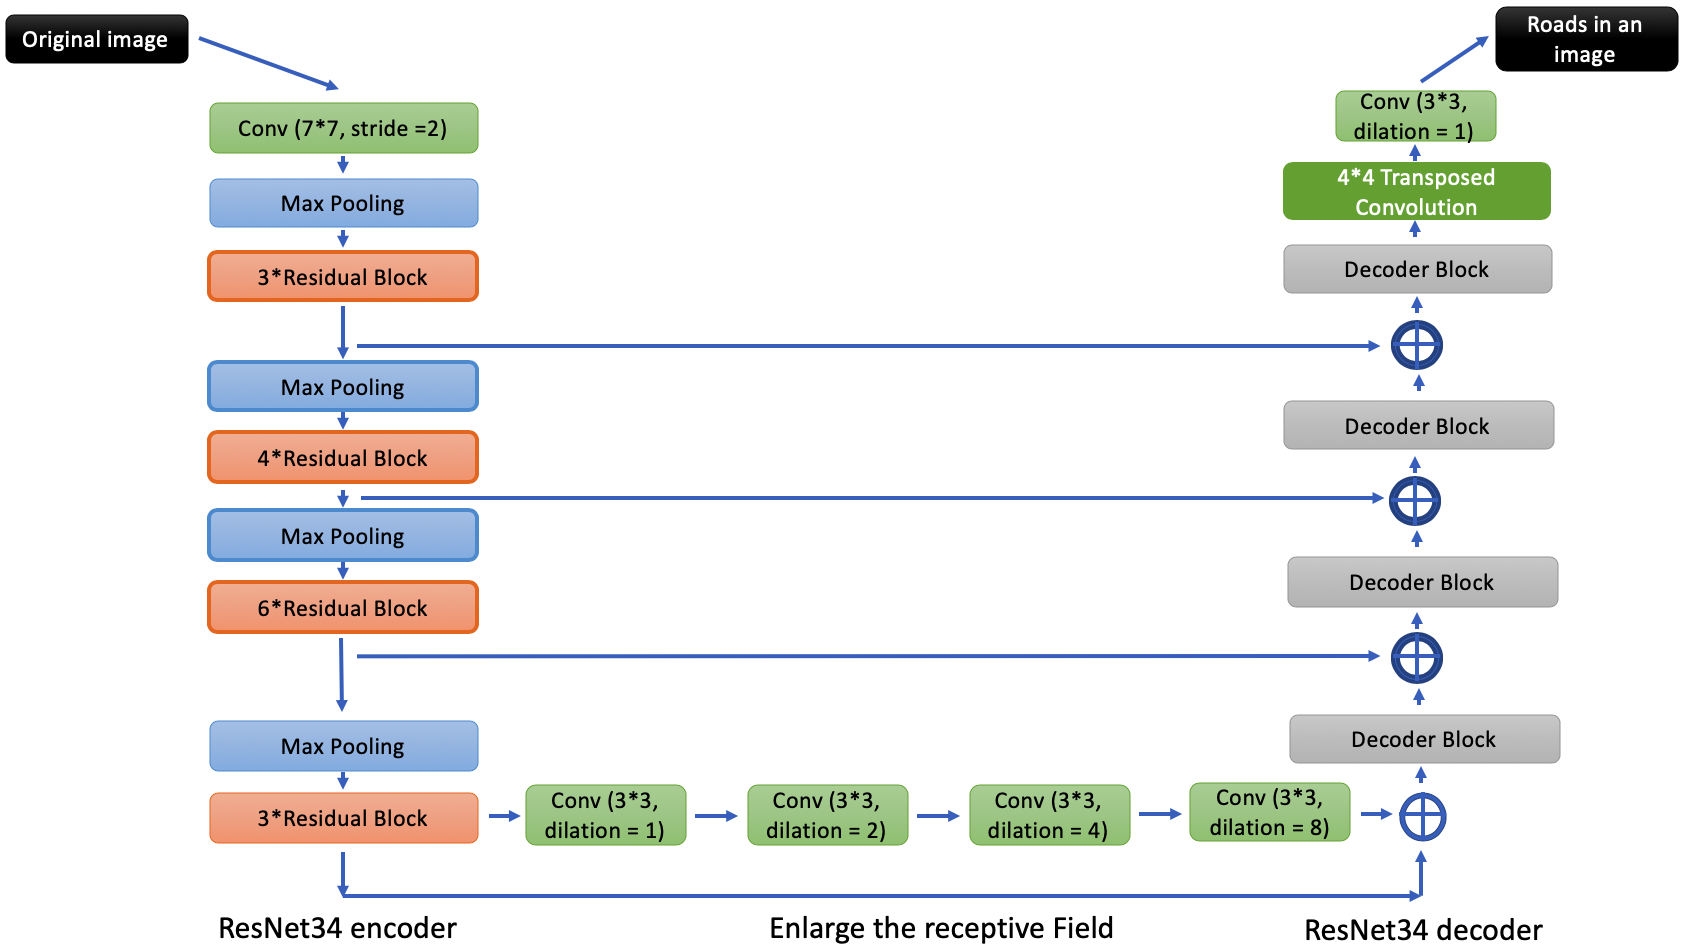
\includegraphics[width=\textwidth]{model_D-LinkNet}
  \caption[Laying out the strucutre for D-LinkNet]{Laying out the strucutre for D-LinkNet~\cite{D-LinkNet}.}
  \label{fig:model_D-LinkNet}
\end{figure}


\textbf{This is how we complete the implementation as given in \cref{chapt:problem} and as shown in \cref{fig:model_complete}.}

\begin{figure}[h!]
  \centering
  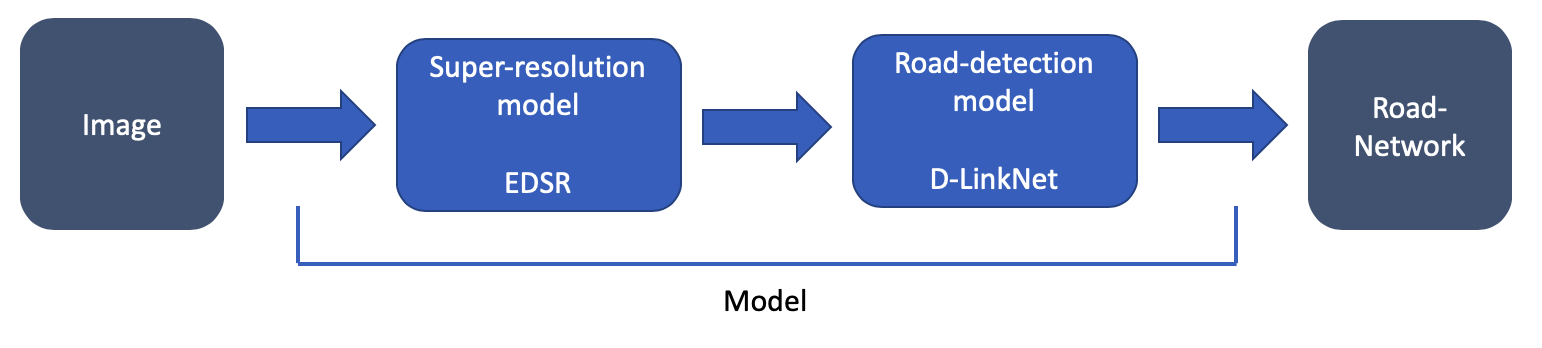
\includegraphics[width=0.8\textwidth]{model_complete}
  \caption{Using EDSR and D-LinkNet together.}
  \label{fig:model_complete}
\end{figure}
\chapter{Handling data for training the model}\label{chapt:data}
\textit{As stated before in \cref{chapt:intro}, Images from Sentinel-2A have been used.}

\section{Get the raw training dataset}
Data needed for training the model is divided into two parts: \textbf{(a)} Satellite image and the \textbf{(b)} Labelled dataset of Roads. Both (a) and (b) should be from the same geography.

Satellite images for Sentinel-2A are available at \url{https://scihub.copernicus.eu/dhus/}. For deep learning, a very accurately labeled dataset is crucial for model training. The pixel-level dataset is challenging to produce in any small community. This is when the web-map services come into the picture. One of the popular mapping services is the Open Street Map~(OSM), which has been widely used to find the road vectors. I will use out satellite images with the road vectors obtained from OSM. An advantage of using OSM is that many human resources are saved, and the main work can be focussed on writing code to validate the research, thus making the process efficient.


\section{Converting data to a usable form}
Even after obtaining the satellite image and road dataset for the same geographical area, the final result image is quite big for Deep Convolutional Neural Network~(DCNN) to handle. To solve this problem, I sliced the image into multiple images of size $544\times544$ (\cref{fig:run_split_images}). This results in multiple small images which can be handled well by a computer (16~GB RAM). This size can be decreased or increased depending on the specifications of the computer used.
\begin{figure}[h!]
  \centering
  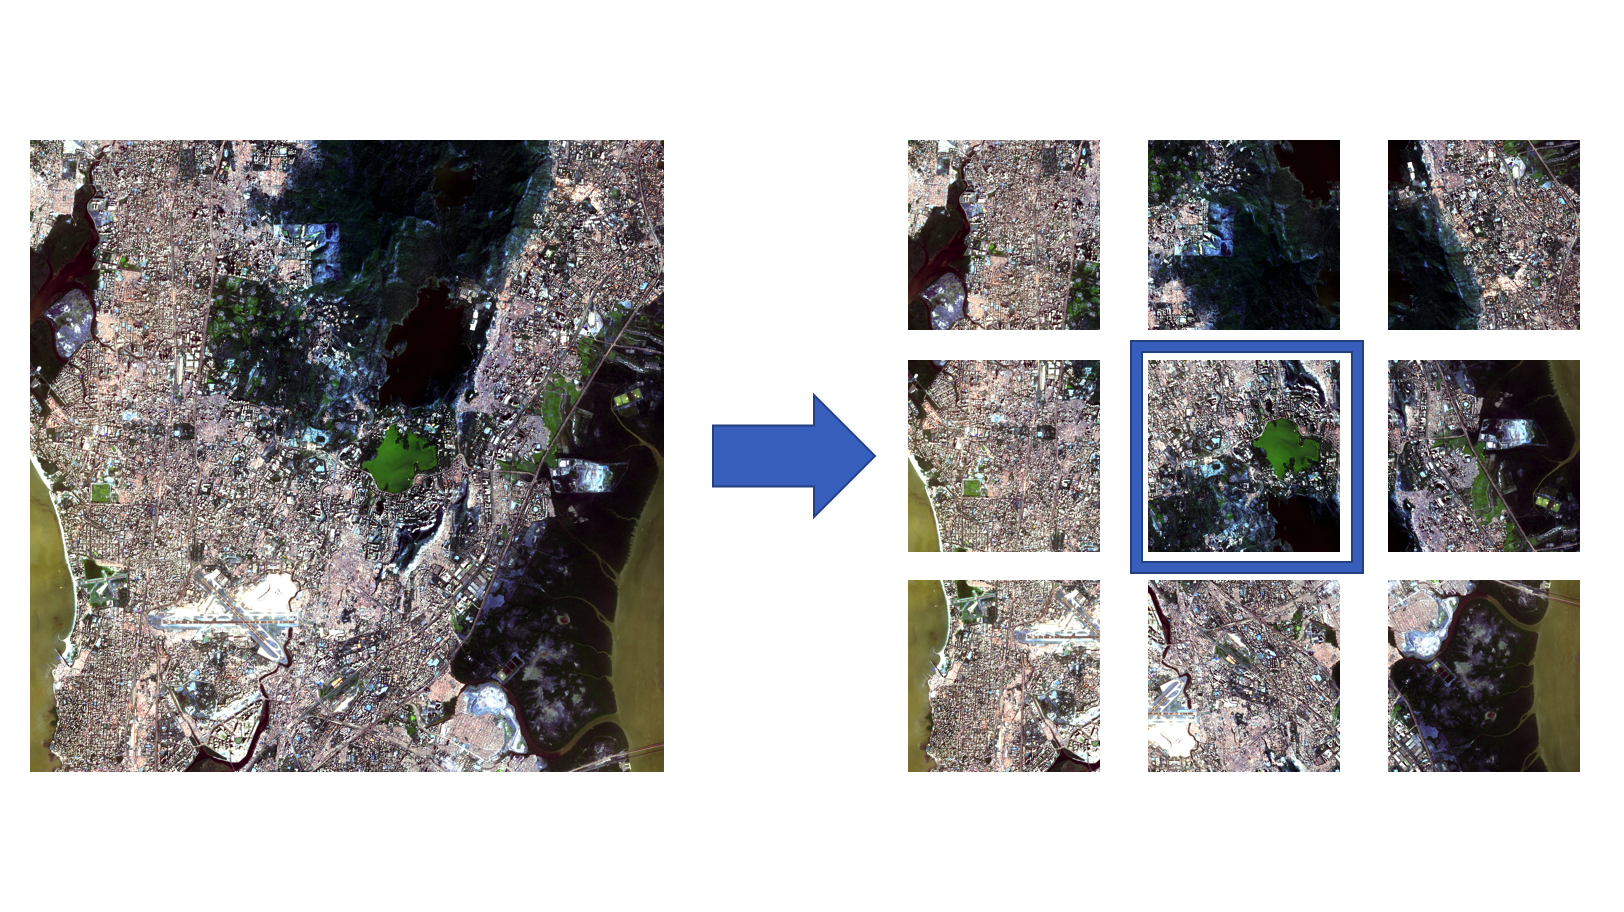
\includegraphics[width=\textwidth]{run_split_image}
  \caption{Image split into 9 parts making it fit for practical use in models.}
  \label{fig:run_split_images}
\end{figure}


\section{Cleaning the obtained dataset}
Though the data is from OSM by multiple collaborators, it is more or less in a raw format and prone to errors. Given its open-source in nature, it may be outdated or, in some cases, need some corrections. These corrections need to be manually done to ensure the training data is accurate before being fed into our model.

The images with less or no roads are removed from the dataset. This is done so that `the-no-road' data should not affect the weights used to identify roads. This step is significant because roads often make up a tiny part of satellite images, and most training images will have no roads on them.


\section{Handling the noise generated to improve training}
Now that the models are chosen, we will now try to link the output of the super-resolution model to the input of road-detector. As specified earlier, our road-detection model assumes the training and input dataset ideally is a pixel-level accurate map. No super-resolution model can be 100 percent accurate, and this becomes the cause of the problem. Thus, this underlying condition needs to be handled to reduce false predictions in the model.

The datasets constructed from a map suffers from two types of labeled noises (\cref{fig:noise_types}):
\begin{itemize}
  \setlength\itemsep{1mm}
  \item Omission noise is when the map is incomplete. It is true for small roads and alleys.
  \item Registration noise is when the location of the object is inaccurate. This noise is quite common, as maintaining pixel-level accuracy is quite difficult to produce.
\end{itemize}

\begin{figure}[h!]
  \centering
  \begin{subfigure}{0.63\textwidth}
    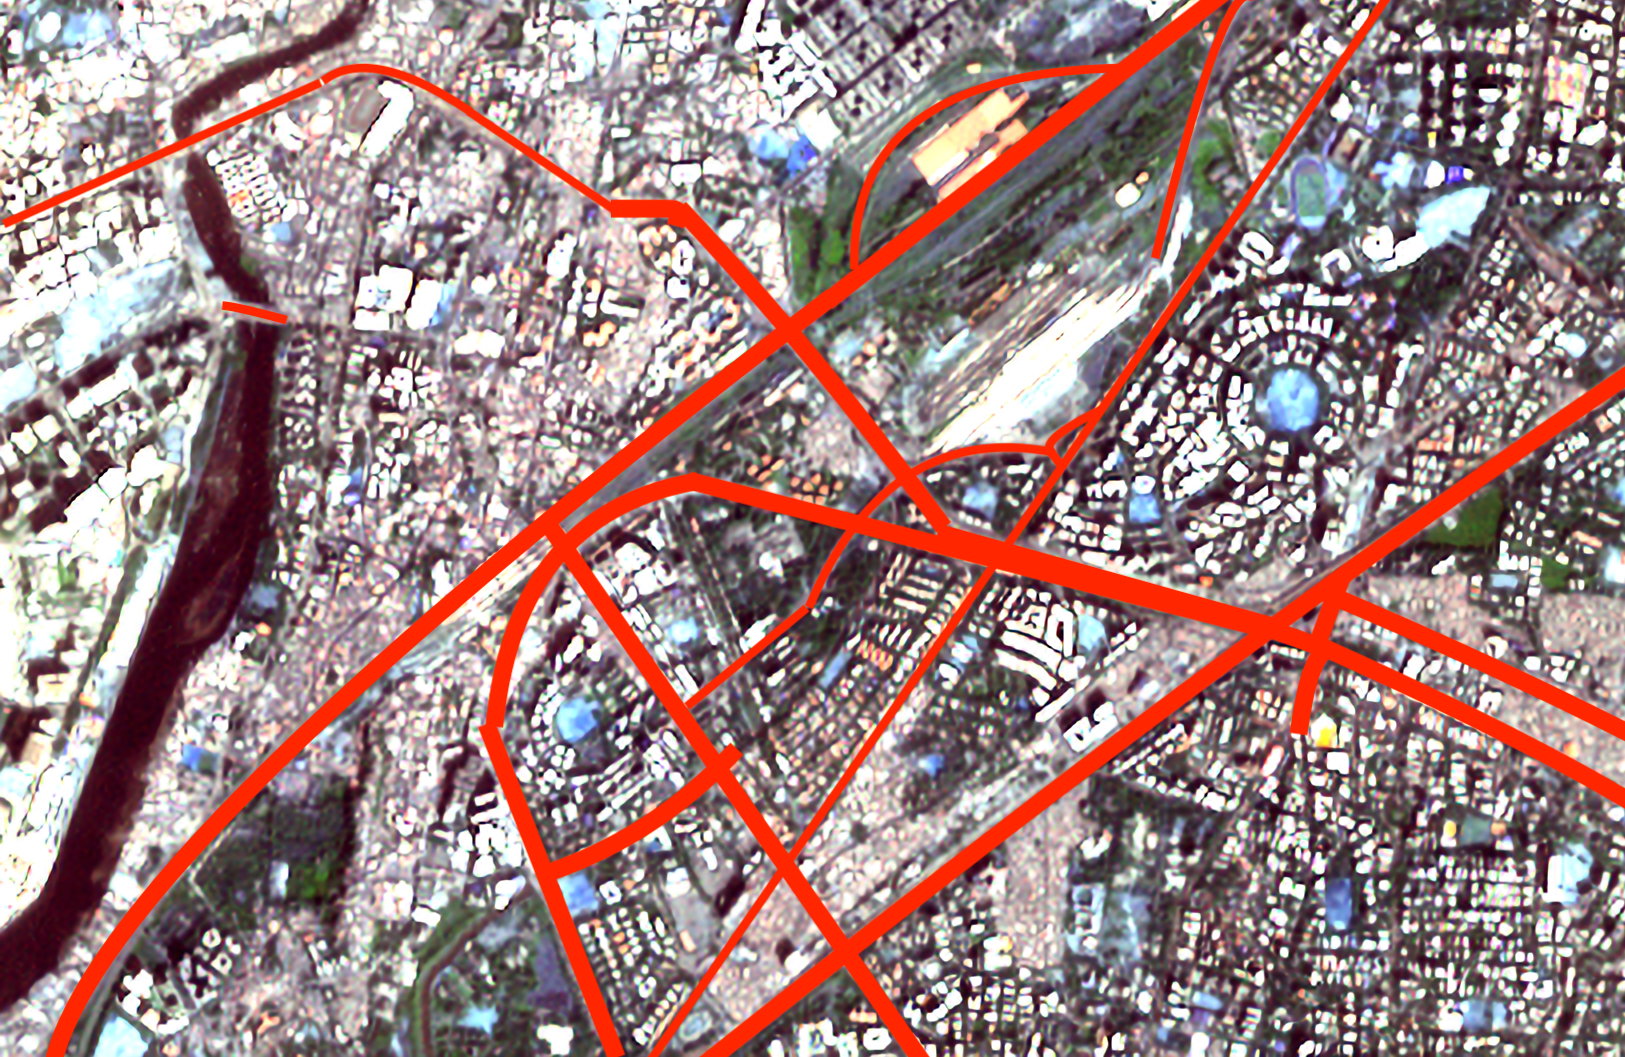
\includegraphics[width=\textwidth]{noise_omission}
    \caption{}
  \end{subfigure}~
  \begin{subfigure}{0.35\textwidth}
    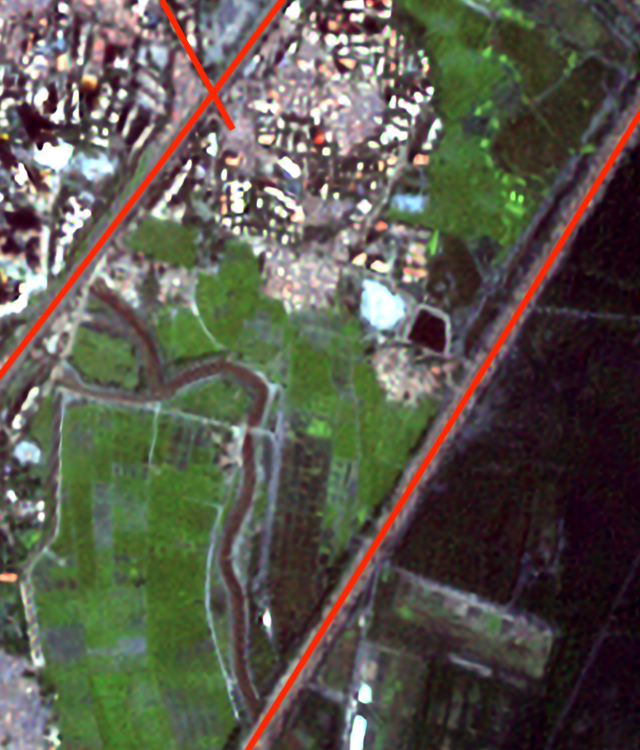
\includegraphics[width=\textwidth]{noise_registration}
    \caption{}
  \end{subfigure}
  \caption[Types of noises in a dataset]{Types of noises in a dataset \textbf{(a)}~Omission noise \textbf{(b)}~Noise registration.}
  \label{fig:noise_types}
\end{figure}

These kinds of errors in the training labels reduce the accuracy of classifiers trained with this data. To solve this, we use a proper loss function during training for our road-detection model.

\chapter{Results}\label{chapt:results}

With so much to talk in this report, everything can be summarised into a small picture - \cref{fig:the_complete_picture}

\section{Pros}
The model predicted most of the roads, which were predicted by the model without super-resolution. Apart from that, the model also predicted a lot of other small roads. On validating with the ground truth images, I found that this was a very good prediction. Checkout \cref{fig:run_merge_road_maps}

\begin{figure}[h!]
  \centering
  \begin{subfigure}{0.55\textwidth}
    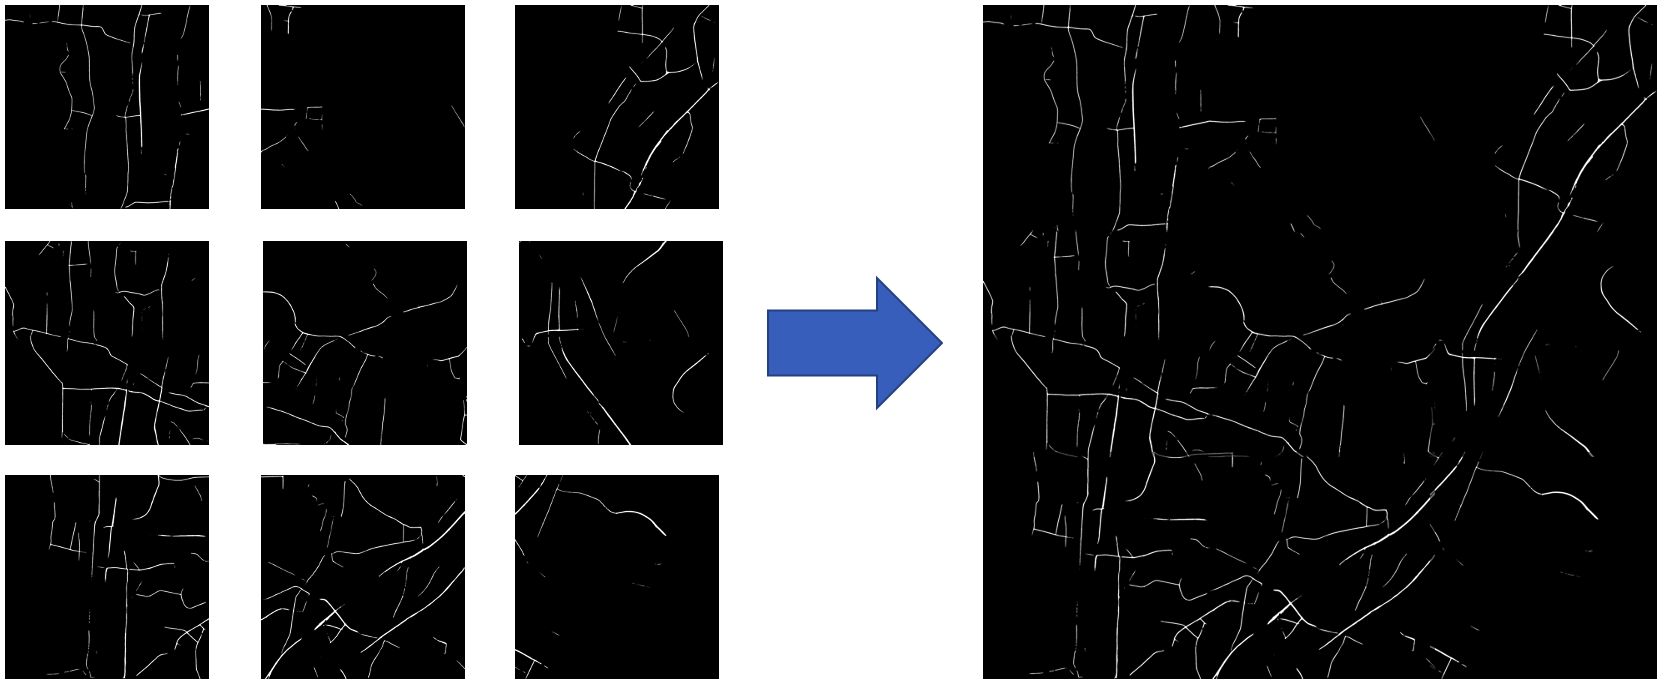
\includegraphics[width=\textwidth]{run_merge_roads}
    \caption{}
  \end{subfigure}~
  \begin{subfigure}{0.21\textwidth}
    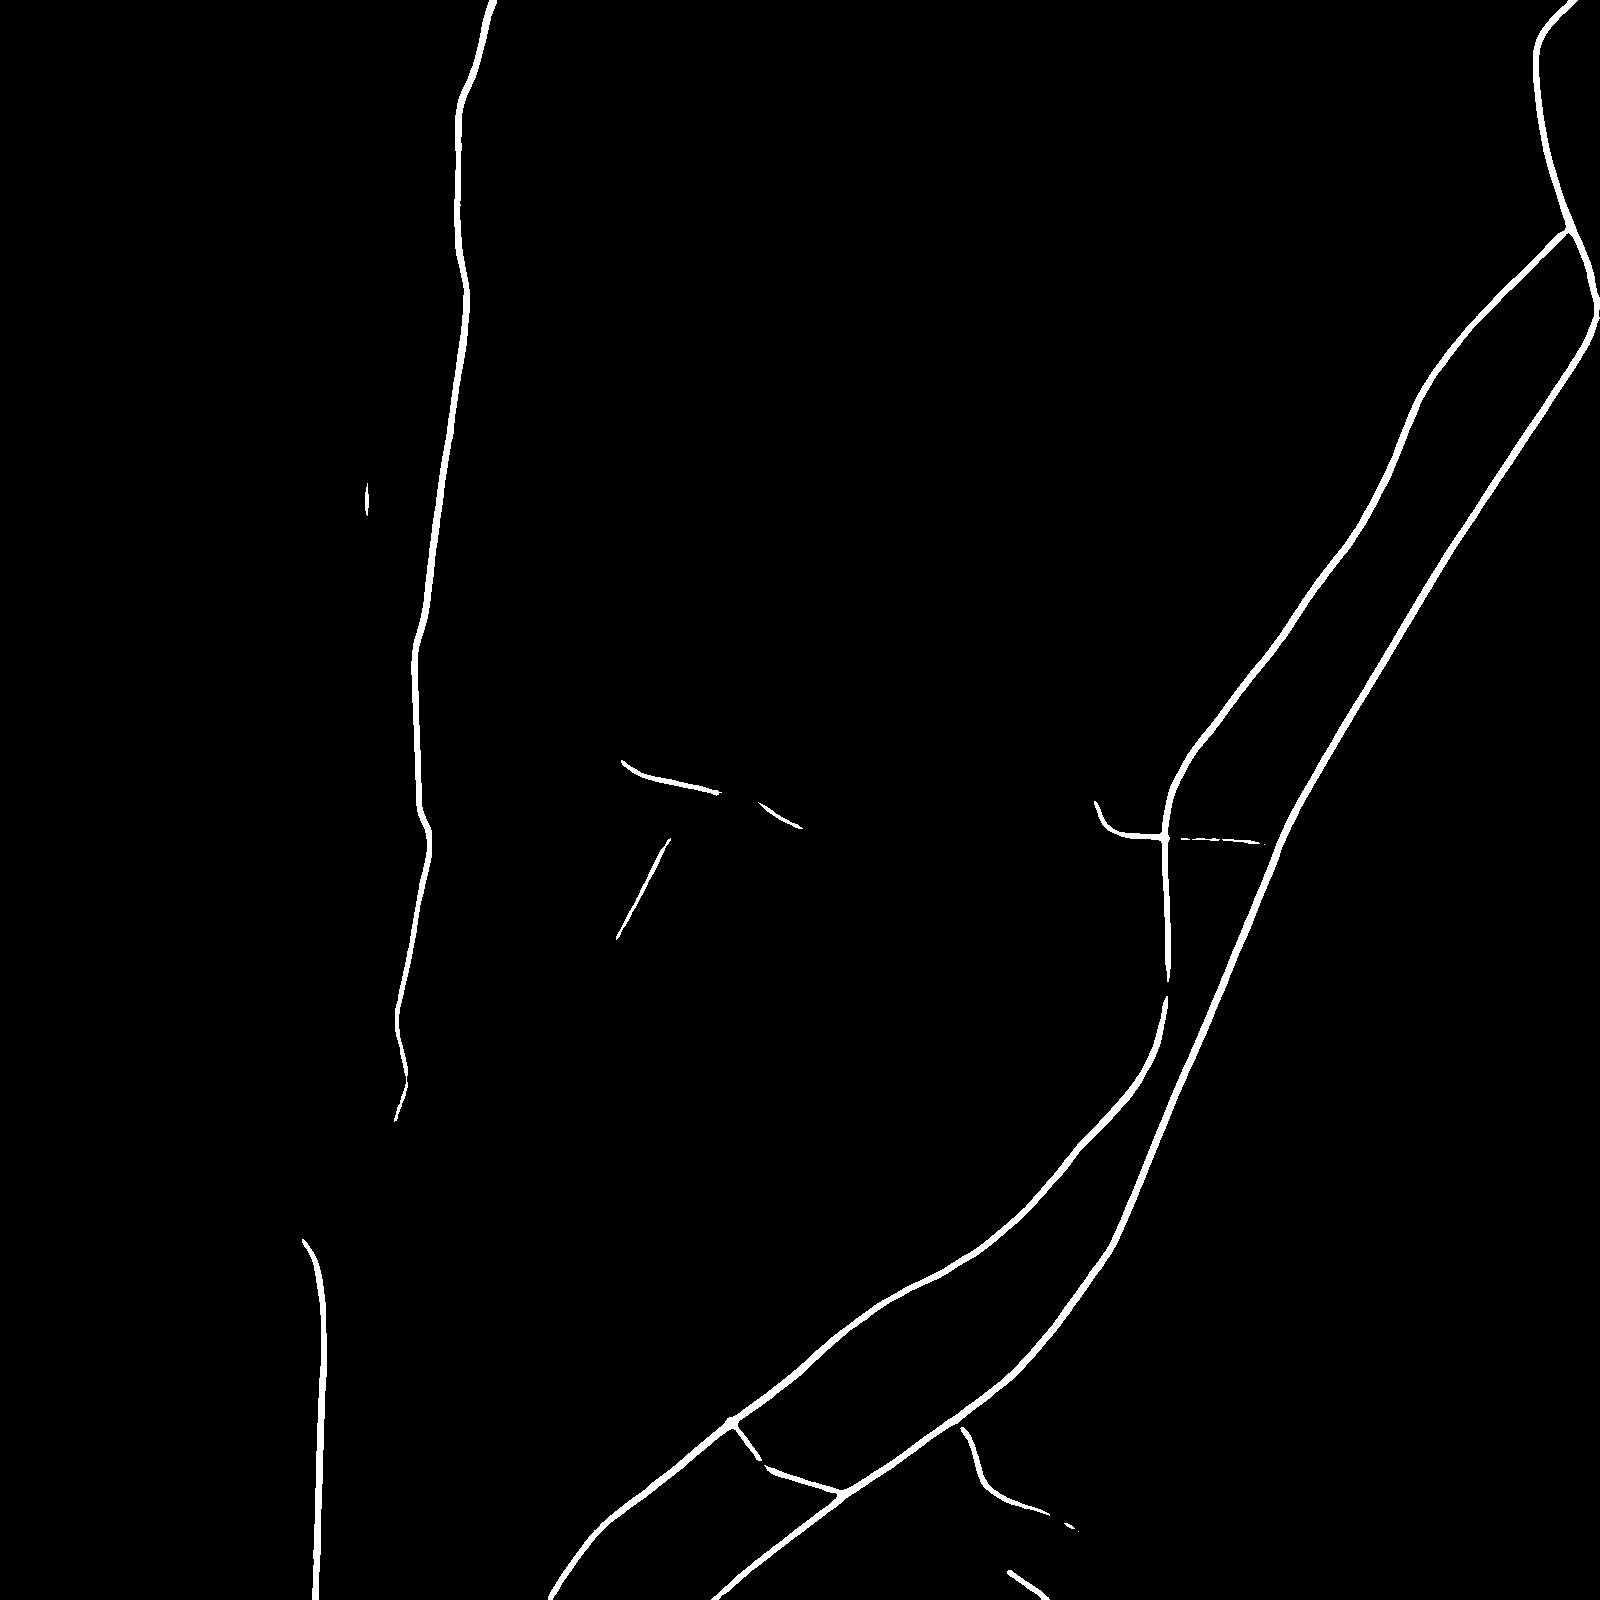
\includegraphics[width=\textwidth]{run_road_linknet}
    \caption{}
  \end{subfigure}~
  \begin{subfigure}{0.21\textwidth}
    \includegraphics[width=\textwidth]{sat_image_run}
    \caption{}
  \end{subfigure}
  \caption[Predictions]{\textbf{(a)} Predictions using our model. \textbf{(b)} Predictions just using the road-detection model. \textbf{(c)} Image used to find predictions. Comparing the original road-detection model with the improved model.}
  \label{fig:run_merge_road_maps}
\end{figure}


\section{Cons}
One of the most noticeable drawbacks of using this model is the amount of time required to get the predictions. 

Another disadvantage is, the model is too much affected due to inaccuracies in the training dataset. If the road gets too thick, say, we take an image with a higher resolution, and run the model; we see that our model has several discontinuities in between. Refer [\cref{fig:cons_coverleaf}]. 
This is mainly because of the noise which has effected the weights. This error can be reduced by training the model with more precise data. Another way to correct this error is to run the algorithm without super-resolution. This means we need to train the model again, this time without super-resolution.

\begin{figure}[h!]
  \centering
  \begin{subfigure}{0.3\textwidth}
    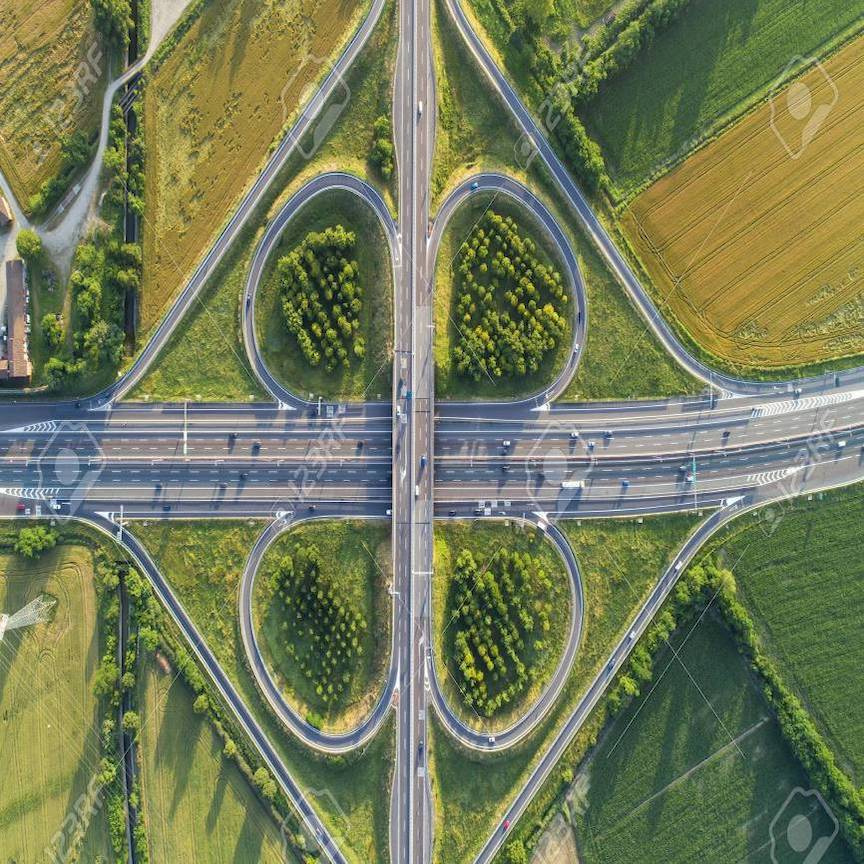
\includegraphics[width=\textwidth]{cons_coverleaf}
    \caption{}
  \end{subfigure}~
  \begin{subfigure}{0.3\textwidth}
    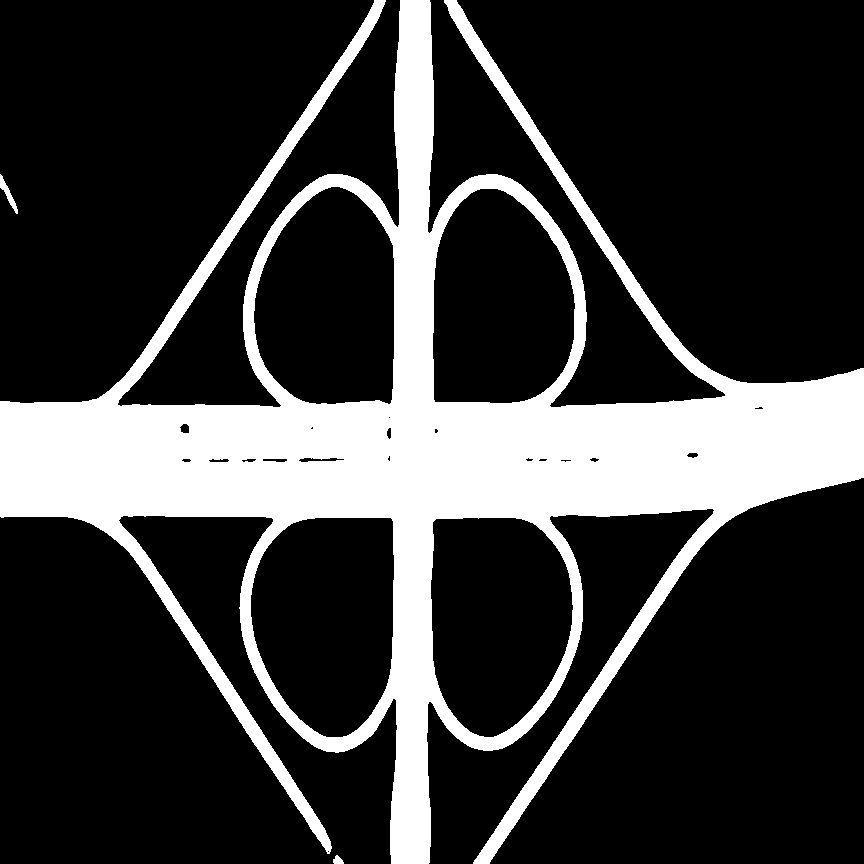
\includegraphics[width=\textwidth]{cons_road_coverleaf}
    \caption{}
  \end{subfigure}~
  \begin{subfigure}{0.3\textwidth}
    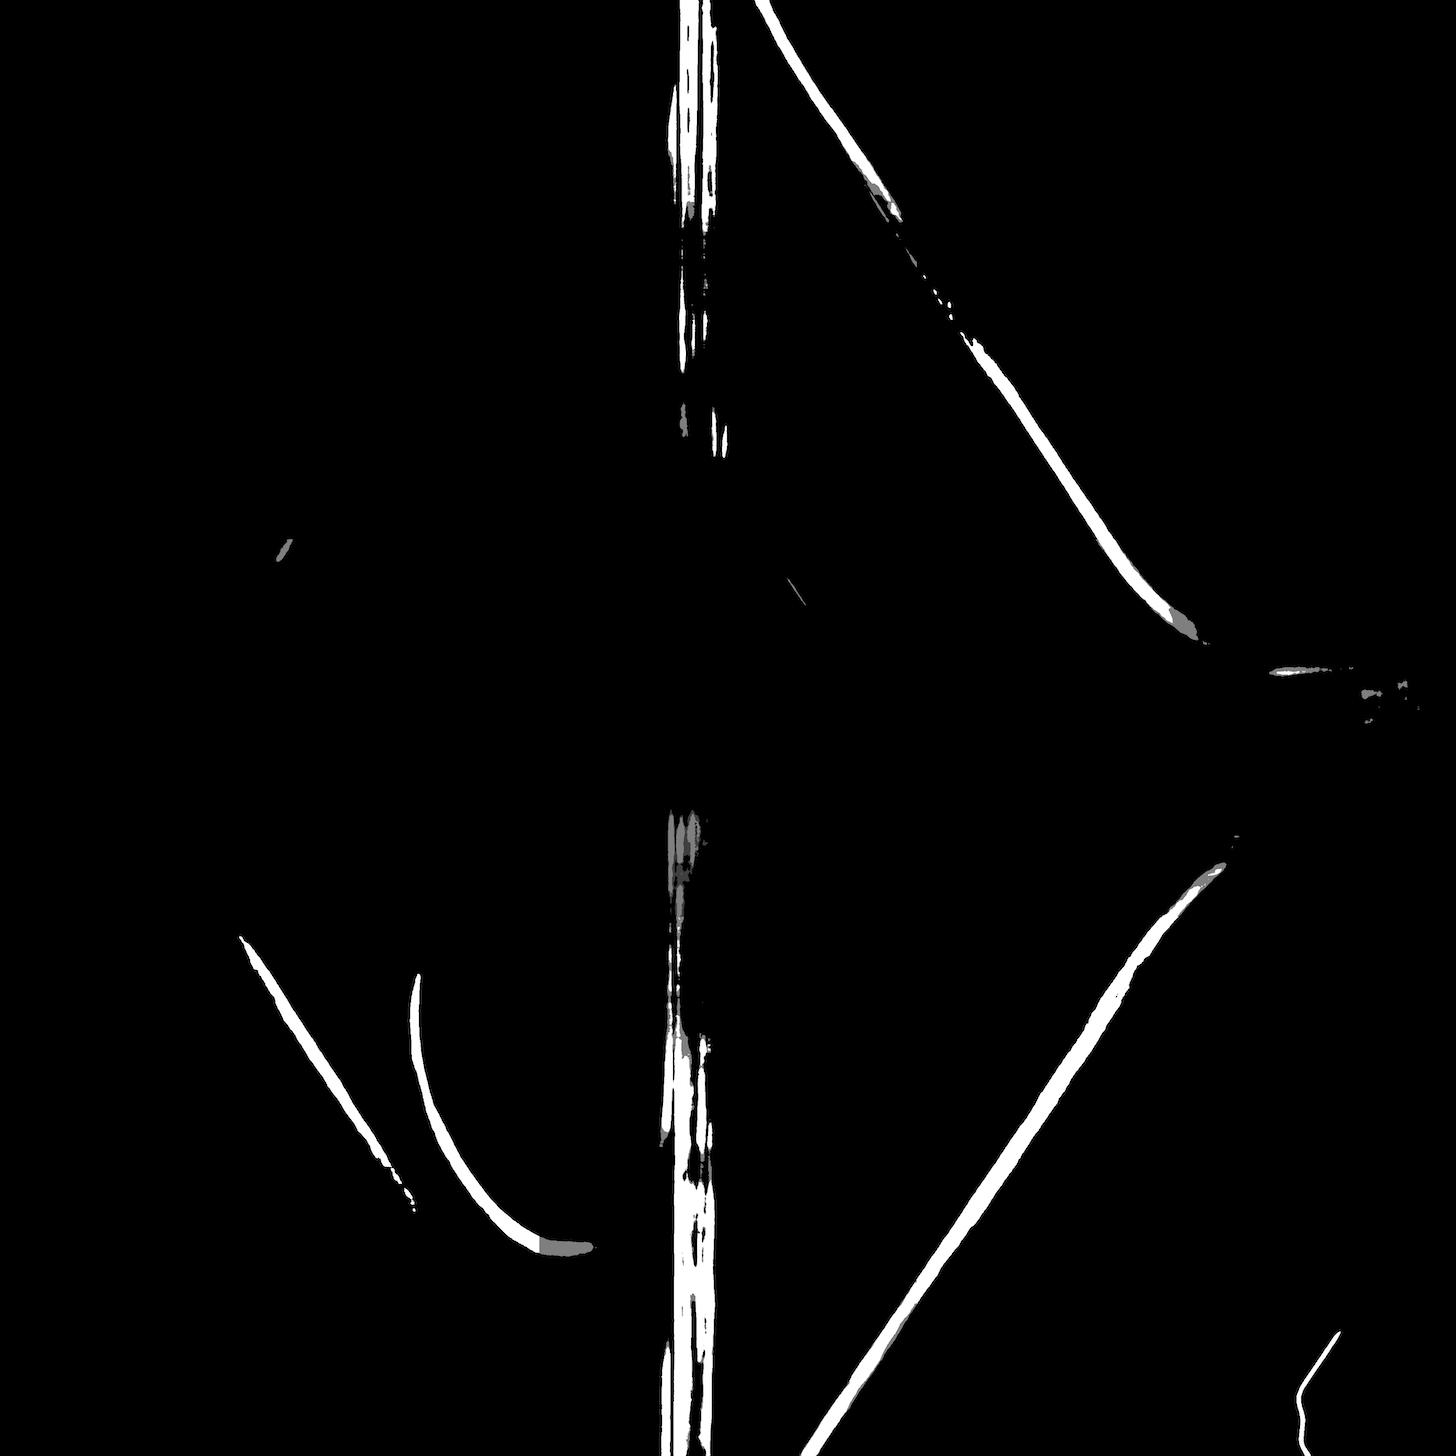
\includegraphics[width=\textwidth]{cons_road_coverleaf_sr}
    \caption{}
  \end{subfigure}
  \caption[Problem in predictions large roads]{\textbf{(a)} The image to apply the model on. \textbf{(b)} Road detection without applying super-resolution. \textbf{(c)} Road detection by out model. When a wide road is to be predicted, the noise takes over and our predictions go horribly wrong.}
  \label{fig:cons_coverleaf}
\end{figure}


Now that we have two predictions, one with super-resolution and without it, we merge them. First, we need to make them of the same resolutions. We do this by finding out the difference factor. Let us say the difference factor is $X$ on each side; we split the lower resolution image pixels into $X$ different pixels on both sides. Then we average the resultant images of the same resolution. For reference: look at \cref{fig:roads_in_confidence}

\begin{figure}[h!]
  \begin{subfigure}[b]{0.25\textwidth}
    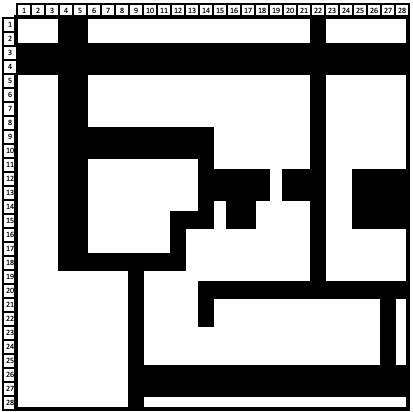
\includegraphics[width=\textwidth]{roads_with_SR}
    \caption{}
  \end{subfigure}~
  \begin{subfigure}[b]{0.15\textwidth}
    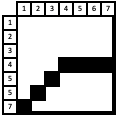
\includegraphics[width=\textwidth]{roads_without_SR}
    \caption{}
  \end{subfigure}~
  \begin{subfigure}[b]{0.25\textwidth}
    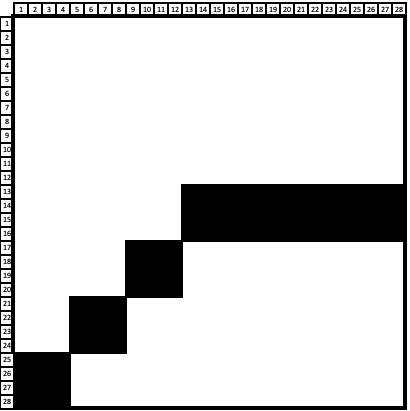
\includegraphics[width=\textwidth]{roads_without_SR_zoomed}
    \caption{}
  \end{subfigure}~
  \begin{subfigure}[b]{0.25\textwidth}
    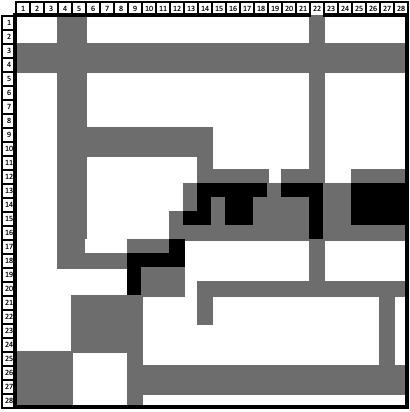
\includegraphics[width=\textwidth]{roads_with_confidence}
    \caption{}
  \end{subfigure}
  \caption[Finding likelihood of roads in predictions]{Merging roads found with \textbf{(a)} Predictions with SR. \textbf{(b)} Predictions without SR. \textbf{(c)} Upscaling of (b). \textbf{(d)} Final result by averaging (a) and (c). Black ones are definitely a road, grey ones having 0.5 probablity of being a road and least likely to find a road on the white pixel.}
  \label{fig:roads_in_confidence}
\end{figure}

\begin{sidewaysfigure}
  \centering
  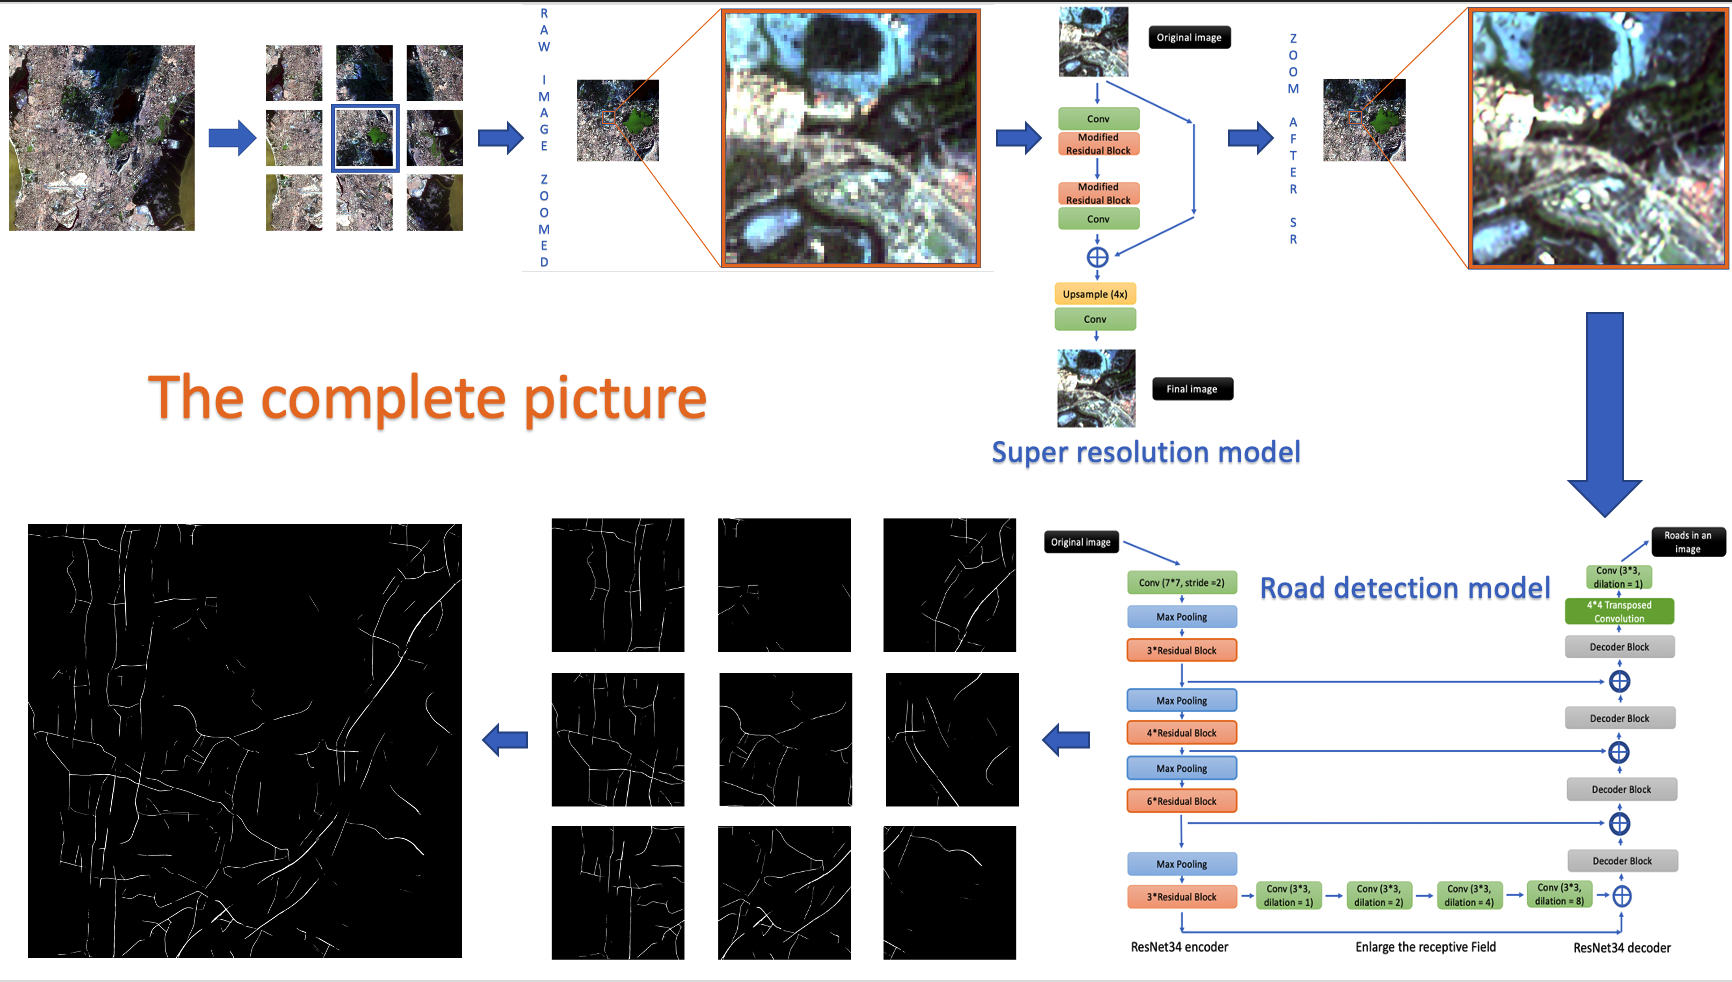
\includegraphics[width=\textheight]{the_complete_picture}
  \caption{A figure summarising the complete process into one}
  \label{fig:the_complete_picture}
\end{sidewaysfigure}

% \chapter{Conclusions}
% \chapter{Scope of Improvements}
% https://towardsdatascience.com/road-segmentation-727fb41c51af
\pagebreak

\begin{appendices}
\chapter{Code}\label{chapt:code}
\textbf{The code can be found at \href{https://nautatva.github.io/btp/code}.}

\section{Summary}
\textbf{Language programmed}: Python 3.8 \bigskip \\
\textbf{General Idea}: The idea is to take an image and apply the concepts of super-resolution. This image, now with the enhanced resolution, is fed into a neural network to identify roads. The benefit of higher resolution means even smaller roads can now be identified. \bigskip \\
\textbf{Constraints}: Each side of the input image must have resolution divisible by 16 for super-resolution and 32 for road-detection.


\section{Notes}
\subsection{Installing GDAL}
A satellite image bit depth is usually 16 bits, and conventional images are 8-bit images. Thus, most of the common python libraries, such as PIL, openCV cannot be used due to information loss. We, therefore, use GDAL and scikit-image libraries to read and write images.

The easiest way to install GDAL is by using anaconda. Install anaconda from \href{https://www.anaconda.com/products/individual#Downloads} and run \mintinline{bash}{conda install -y gdal} on command line~(CMD) or terminal.


\subsection{Read and write an image}
Using GDAL can be tricky. Therefore, \texttt{`helper.py'} has the functions \texttt{read\_image} and \texttt{write\_image}. These take care of the possible corner-cases which may arise so that the libraries can be used easily without any problems. An extra function \texttt{`convertTo8Bit'} can be used to convert any image into 8 Bits.

\begin{minted}{python}
import helper

image_array = read_image('path_to_image')  # Reads image and stores the matrix in image variable; Lets say 16Bit image
write_image(image_array, 'output.png')  # Writes the image array to a file named output.png
convertTo8Bit('path_to_image', 'output_8bit.png')
\end{minted}


\subsection{Splitting large image into smaller chunks}
To ensure the image can be processed on a personal computer, we use the \texttt{`image.split()'} to divide the given image into multiple parts of a specified size.

\begin{minted}{python}
df = image.split('source', path(root_path, 'sliced'))  # df contains all the details of the smaller images. These small images are stored in the `sliced` directory
\end{minted}

\subsection*{Input}
\begin{itemize}
  \setlength\itemsep{1mm}
  \item The split function takes in an image or a folder path containing images and folder path for output as input.
  \item Optional parameters are SliceX and SliceY, whose default values are both 544. It is the dimension of the image we want for each chunk.
  \item Other optional parameters are StrideX and StrideY, which set the value of the image to be slid after cropping up. Default values are set to be 540 for both.
\end{itemize}

\subsection*{Output}
\begin{itemize}
  \setlength\itemsep{1mm}
  \item The function returns an array with the details of how the image is split.
  \item The files are always of dimension $SliceX\times SliceY$.
  \item The name convention for images saved is \newline
    nameOfImage\_\_InitialY\_InitialX\_sliceHeight\_sliceWidth\_padding\_TotalWidth\_TotalHeight \newline
    (with the required extension).
\end{itemize}


\subsection*{Example}
\begin{itemize}[label={}]
  \item\textbf{Input}:
  \begin{itemize}[{\textbullet}]
    \setlength\itemsep{1mm}
    \item \textbf{Name of Image}: coverleaf.jpg
    \item \textbf{Stride X}: 540
    \item \textbf{Stride Y}: 540
    \item \textbf{SliceX}: 544
    \item \textbf{SliceY}: 544
  \end{itemize}

  \item\textbf{Property of image}:
  \begin{itemize}[{\textbullet}]
    \setlength\itemsep{1mm}
    \item Width of image: 864
    \item Height of image: 864
  \end{itemize}

  \item\textbf{The output files are named}:
  \begin{itemize}[>]
    \setlength\itemsep{1mm}
    \item coverleaf\_\_0\_0\_544\_544\_0\_864\_864
    \item coverleaf\_\_0\_320\_544\_544\_0\_864\_864
    \item coverleaf\_\_320\_0\_544\_544\_0\_864\_864
    \item coverleaf\_\_320\_320\_544\_544\_0\_864\_864
  \end{itemize}
\end{itemize}
\section{Super Resolution}
For applying super-resolution on one image, use \texttt{`apply\_sr'}. When applying SR on multiple images, copy them into a folder, and use \texttt{`batch\_SR'}. You can download my trained weights from \href{https://nautatva.github.io/btp/weight/sr}{here}.

\begin{minted}{python}
# Use depending on the need
from super_resolution import apply_SR, batch_SR


# SR on single image:
apply_SR('path_image_in', 'path_image_out', 'path_to_SR_weight')

# SR on multiple images:
batch_SR('folder_path_in', 'folder_path_out', 'extensions_of_files to be processed', 'path_to_SR_weight')
\end{minted}


\section{Road-detection}
Apply road detection using the \texttt{`find\_roads'} function. It takes in a folder and detects the road in every file of that folder. You can download my trained weights from \href{https://nautatva.github.io/btp/weight/road}{here}.

\begin{minted}{python}
# Find roads
find_roads(source=path(root_path, "sr"), output=path(root_path, "roads"), weights="path_to_weights")  # Takes in the source folder sr, predicts roads in the image and writes the image in folder named roads.
\end{minted}

\section{Merge the split images}
Merging the images to get back the roads on the entire map is done by the \texttt{`image.merge'} function.
Set the scale to the factor of resolution change during super-resolution.

\begin{minted}{python}
merge('input_folder', 'output_folder', 'extension_of_files_to_be_joined', "scale_SR")
\end{minted}
\end{appendices}
\normalem
\bibliographystyle{unsrtnat} 
%\bibliography{longnamesfirst,semicolon}
\addcontentsline{toc}{chapter}{\numberline{}Bibliography}
\bibliography{bibliography}

% % Adding a bibliography if citations are used in the report
% \bibliographystyle{plain}
% \bibliography{bibliography.bib}
% % Adds reference to the Bibliography in the ToC
% \addcontentsline{toc}{chapter}{\bibname}
% % \printbibliography

% [1]: Arin Basu. (April 16 2017). How to add footnotes https://medium.com/@arinbasu/you-can-use-footnotes-thus-babus%C2%B9-6c485c4eff1e

\pagebreak

% \chapter*{Appendix A: Resources}
% [\textit{Report the config files of the software used (i.e. SU2 \cite{economon2015su2} and the mesher). Also attach to this report an archive with the mesh files, solutions and the reference solution data (e.g. data points of a Cp plot ...)}]
% \section*{Mesh configuration files}
% \section*{SU2 configuration files}
% \section{Reference solution data}


\end{document}